\section{Thí nghiệm}
\label{sec:experiments}

Để chứng minh tính hiệu quả của phương pháp tiếp cận tổng thể và phương pháp QCAD được đề xuất, chúng tôi tiến hành thử nghiệm trên nhiều bộ dữ liệu tổng hợp và thực tế. Trước tiên, chúng tôi sẽ giải thích các lựa chọn liên quan đến bộ dữ liệu, thuật toán cơ bản và tiêu chí đánh giá, sau đó chúng tôi trình bày cả kết quả định lượng và nghiên cứu điển hình để điều tra khả năng diễn giải và tiện ích thực tế.

Ngoài ra, chúng tôi chứng minh tính mạnh mẽ của QCAD liên quan đến "số lượng siêu tham số lân cận gần nhất bằng phương pháp phân tích độ nhạy và tiến hành một số nghiên cứu cắt bỏ để điều tra tác động của siêu tham số". Vì lý do không gian và sự ngắn gọn, việc phân tích độ nhạy và
nghiên cứu cắt bỏ được đưa ra trong Phụ lục~\ref{Appendix:Sensitivity} và~\ref{Appendix:Ablation}.

\subsection{Dữ liệu}
\label{subsec:datasets}

Việc đánh giá các thuật toán phát hiện bất thường không được giám sát là một thách thức do thiếu dữ liệu điểm chuẩn được thống nhất chung và các bộ dữ liệu phân loại lấy mẫu xuống đã bị chỉ trích vì sự thay đổi về bản chất của các ngoại lệ thu được \citep{farber2010using,campos2016evaluation}.

Khi đánh giá các thuật toán phát hiện bất thường theo ngữ cảnh \emph{không giám sát}, vấn đề này càng trở nên phức tạp hơn do yêu cầu phải có cả các đặc trưng ngữ cảnh và hành vi, đồng thời---quan trọng hơn---xử lý các tính năng đó một cách khác nhau \citep{liang2016robust}. Do đó, một cách tiếp cận được chấp nhận rộng rãi là đưa các điểm bất thường theo ngữ cảnh vào các tập dữ liệu hiện có một cách giả tạo bằng cách sử dụng sơ đồ nhiễu loạn.

\subsubsection{Tiền xử lý dữ liệu}
\label{prelim:gower}

Để làm cho các bộ dữ liệu phù hợp với tất cả các phương pháp phát hiện điểm bất thường, chúng ta cần xử lý trước chúng trước khi đưa vào các điểm bất thường theo ngữ cảnh. Đầu tiên, chúng tôi tận dụng Mã hóa nhãn \citep{seger2018investigation} để chuyển đổi các đặc điểm ngữ cảnh phân loại thành dạng số. Thứ hai, chúng tôi sử dụng chuẩn hóa Min-Max để mở rộng tất cả các đặc trưng hành vi thành $[0,1]$. Chuẩn hóa Min-Max được sử dụng thường xuyên trong nhiều hoạt động phát hiện bất thường và thường cải thiện hiệu suất \citep{kandanaarachchi2020normalization}.\textbf{Khoảng cách của Gower} Để có thể tính toán độ tương tự giữa hai điểm dữ liệu chứa cả đặc điểm phân loại và số, chúng ta có thể sử dụng khoảng cách \citep{gower1971general} của Gower. Cụ thể, khoảng cách của Gower giữa các điểm dữ liệu $\mathbf{c}_{i} = (c_{i}^{1},...,c_{i}^{p},...c_{i}^{P})$ và $\mathbf{c}_{j} = (c_{j}^{1},...,c_{j}^{p},...c_{j}^{P})$ được xác định là $1- \frac{1}{P}\sum_{p=1}^{P}ps_{ij}^{p}$, trong đó $ps_{ij}^{p}$ thể hiện sự tương đồng một phần giữa các phiên bản dữ liệu $\mathbf{c}_{i}$ và $\mathbf{c}_{j}$ trong chiều thứ $p$. Đối với đối tượng số, $ps_{ij}^{p} = 1- \frac{\abs{c_{i}^{p}-c_{j}^{p}}}{\mathrm{max}(\mathbf{c}^p)-\mathrm{min}(\mathbf{c}^p)}$, với $\mathrm{max}(\mathbf{c}^p)$ và $\mathrm{min}(\mathbf{c}^p)$ lần lượt biểu thị giá trị tối đa và tối thiểu của tất cả các điểm dữ liệu cho đối tượng địa lý $p$-th. Đối với tính năng phân loại, $ps_{ij}^{p} = \mathbb{I}(c_{i}^p-c_{j}^p$), trong đó $\mathbb{I}(\cdot)$ đại diện cho chức năng chỉ báo. Do đó, khoảng cách của Gower giữa hai điểm dữ liệu luôn nằm trong $[0,1]$, với giá trị thấp hơn biểu thị mức độ tương tự lớn hơn.

\subsubsection{Lược đồ nhiễu loạn cho việc tiêm ngoại lệ}

\cite{song2007conditional} đã đề xuất một sơ đồ nhiễu loạn để đưa các điểm bất thường theo ngữ cảnh vào các tập dữ liệu không có điểm bất thường trên cơ sở thực tế, đã trở thành một tiêu chuẩn thực tế để đánh giá khả năng phát hiện điểm bất thường theo ngữ cảnh~\citep{song2007conditional, liang2016robust, zheng2017contextual, calikus2021wisdom}.



Tuy nhiên, sơ đồ nhiễu loạn này cũng bị chỉ trích vì hai lý do~\citep{song2007conditional,kuo2018detecting}.
Đầu tiên, các đối tượng thu được bằng cách hoán đổi các giá trị đặc trưng vẫn có khả năng là bình thường về mặt ngữ cảnh. Thứ hai, một số loại dị thường rất phổ biến không thể được giải quyết thông qua sơ đồ nhiễu loạn này. Ví dụ: người ta không thể thu được các giá trị cực trị bằng cách hoán đổi các giá trị đặc trưng trong một tập dữ liệu sạch, trong khi hầu hết các phương pháp phát hiện bất thường đều cho rằng tập dữ liệu huấn luyện không bị nhiễm bẩn. Để tránh những vấn đề này, \cite{kuo2018detecting} đã giới thiệu một sơ đồ nhiễu loạn khác để tạo ra các dị thường. Chúng tôi phát triển một sơ đồ nhiễu loạn mới bằng cách cải tiến sơ đồ này như sau.Với tập dữ liệu $\mathbf{X}$ chứa các phiên bản dữ liệu $N$ với bộ đặc trưng ngữ cảnh $\mathbf{C} = \{\mathbf{c}^{1},...,\mathbf{c}^{P}\}$ và bộ đặc trưng hành vi $\mathbf{B} = \{\mathbf{b}^{1},...,\mathbf{b}^{Q}\}$, trước tiên chúng tôi sử dụng chuẩn hóa Min-Max để chia tỷ lệ các đặc trưng hành vi của tất cả các đối tượng thành $[0,1]$ (giữ nguyên các đặc trưng ngữ cảnh), dẫn đến một tập dữ liệu mới $\Tilde{\mathbf{X}}$. Thứ hai, để đưa các dị thường $m$ vào $\Tilde{\mathbf{X}}$, với $0<m \ll N$, chúng tôi chọn ngẫu nhiên các đối tượng $m$ $\mathbf{x}_{1},\ldots,\mathbf{x}_{m}$ một cách thống nhất từ ​​$\Tilde{\mathbf{X}}$. Đối với mỗi $\mathbf{x} =(\mathbf{c},\mathbf{b})$ trong $\Tilde{\mathbf{X}}$, $\mathbf{c}$ biểu thị các giá trị đặc trưng ngữ cảnh và $\mathbf{b}$ biểu thị các giá trị đặc trưng hành vi. Thứ ba, đối với đối tượng được chọn $\mathbf{x}_{i} = (\mathbf{c}_{i}, \mathbf{b}_{i})= (c^{1}_{i},...,c^{p}_{i},...,c^{P}_{i},b^{1}_{i},...,b^{q}_{i},...,b^{Q}_{i})$ và đặc trưng hành vi $\mathbf{b}^{q}$, chúng tôi lấy mẫu một số ngẫu nhiên thống nhất từ ​​$[-0.5,-0.1] \bigcup [0.1,0.5]$, sau đó thêm số ngẫu nhiên này vào giá trị đặc trưng hành vi của $\mathbf{x}_{i}$, cụ thể là $b^{q}_{i}$, tạo ra $\hat{b}^{q}_{i}$. Theo cách tương tự, chúng tôi lặp lại quy trình này cho từng đặc trưng hành vi, tạo ra $(\hat{b}^{1}_{i},...,\hat{b}^{Q}_{i})$ hoặc $\hat{\mathbf{b}}_{i}$. Theo đó, chúng ta tạo ra một đối tượng mới
$\tilde{\mathbf{x}} = (\mathbf{c}, \hat{\mathbf{b}})$ là sự bất thường theo ngữ cảnh. Thứ tư, chúng tôi lặp lại bước thứ ba cho từng đối tượng được chọn, dẫn đến các đối tượng bị nhiễu loạn $m$.
Thứ năm và cuối cùng, chúng tôi thay thế các đối tượng đã chọn trong tập dữ liệu gốc bằng các đối tượng nhiễu loạn tương ứng của chúng. Để cho phép chèn các giá trị cực trị, chúng tôi cố tình không cắt bớt các giá trị bên ngoài $[0,1]$ sau khi thêm một số ngẫu nhiên vào từng đặc trưng hành vi.

Sơ đồ nhiễu loạn của chúng tôi có những ưu điểm sau. Khi so sánh với sơ đồ nhiễu loạn hoán đổi do \cite{song2007conditional} đề xuất, các đối tượng thu được từ sơ đồ nhiễu loạn của chúng tôi rất khó có thể duy trì trạng thái bình thường theo ngữ cảnh. Ngoài ra, sơ đồ nhiễu loạn của chúng ta có thể---nhưng không phải lúc nào cũng---dẫn đến các giá trị cực trị. Lưu ý rằng chúng tôi không tuân thủ nghiêm ngặt sơ đồ nhiễu loạn do \cite{kuo2018detecting} đề xuất vì phương pháp của họ chỉ thêm một số không âm vào các đặc trưng hành vi. Một mặt, đôi khi số không âm này bằng 0, dẫn đến việc tiêm vào một vật thể bình thường là ``dị thường'. Mặt khác, đôi khi con số không âm này rất lớn, khiến đối tượng được tiêm (cũng) dễ bị phát hiện. Sơ đồ nhiễu loạn của chúng tôi tránh được những vấn đề này bằng cách trước tiên bình thường hóa các giá trị đặc trưng hành vi, sau đó thiết lập các giới hạn trên và dưới hợp lý hơn cho nhiễu loạn.

\subsubsection{Bộ dữ liệu}

Để đánh giá và so sánh phương pháp của chúng tôi trên nhiều loại bộ dữ liệu khác nhau, chúng tôi tạo bộ dữ liệu tổng hợp $10$ và chọn bộ dữ liệu trong thế giới thực $20$; các thuộc tính của chúng được tóm tắt lần lượt trong các Bảng~\ref{tab:data_summary1} và \ref{tab:data_summary2}.\begin{table}[!htbp]
	\caption{Tóm tắt các bộ dữ liệu tổng hợp. $\#Num, \#Cat, \#\mathbf{C}$ và $\#\mathbf{B}$ lần lượt biểu thị số lượng đối tượng số, số lượng đối tượng phân loại/danh nghĩa, số lượng đối tượng theo ngữ cảnh và số lượng đối tượng hành vi. Tất cả các đặc trưng hành vi đều là số, các đặc điểm ngữ cảnh có thể được trộn lẫn.}
	\centering
	\begin{tabular}{cccccc}
		\toprule
		Bộ dữ liệu &Sơ đồ & \#Num & \#Cat & \#$\mathbf{C}$ & \#$\mathbf{B}$ \\
		\midrule
		Syn1 & S1 & 8 & 2 & 5 & 5 \\
		\midrule
		Syn2 & S2 & 8 & 2 & 5 & 5 \\
		\midrule
		Syn3 & S3 & 8 & 2 & 5 & 5 \\
		\midrule
		Syn4 & S4 & 8 & 2 & 5 & 5 \\
		\midrule
		Syn5 & S5 & 8 & 2 & 5 & 5 \\
		\midrule
		Syn6 & S1 & 19 & 6 & 20 & 5 \\
		\midrule
		Syn7 & S2 & 19 & 6 & 20 & 5 \\
		\midrule
		Syn8 & S3 & 19 & 6 & 20 & 5 \\
		\midrule
		Syn9 & S4 & 19 & 6 & 20 & 5 \\
		\midrule
		Syn10 & S5 & 19 & 6 & 20 & 5 \\
		\bottomrule
	\end{tabular}
	\label{tab:data_summary1}
\end{table}

Đầu tiên chúng ta thảo luận về dữ liệu tổng hợp. Để có thể tạo ra dữ liệu với nhiều dạng và mức độ phụ thuộc khác nhau giữa các đặc trưng hành vi và ngữ cảnh, chúng tôi đề xuất các sơ đồ tạo sau. Đối với $q \in \{1,...,Q\}$, chúng tôi có
\begin{itemize}
    \item[(S1)] $\mathbf{b}^{q} = \sum_{p=1}^{Q}\left(\alpha_{qp}\cdot\mathbf{c}^{p}\right)+\boldsymbol{\epsilon}$;
    \item[(S2)] $\mathbf{b}^{q} = \sum_{p=1}^{Q}\left(\alpha_{qp}\cdot(\mathbf{c}^{p})^{3}\right)+\boldsymbol{\epsilon}$,
    \item[(S3)] $\mathbf{b}^{q} = \sum_{p=1}^{Q}\left(\alpha_{qp}\cdot\mathrm{sin}(\mathbf{c}^{p})\right)+\boldsymbol{\epsilon}$,
    \item[(S4)] $\mathbf{b}^{q} = \sum_{p=1}^{Q}\left(\alpha_{qp}\cdot\mathrm{log}(\mathbf{1}+\vert\mathbf{c}^{p}\vert)\right)+\boldsymbol{\epsilon}$,
    \item[(S5)] $\mathbf{b}^{q} = \sum_{p=1}^{Q}\left(\alpha_{qp}\cdot\mathbf{c}^{p}+\beta_{qp}\cdot(\mathbf{c}^{p})^{3}+\gamma_{qp}\cdot\mathrm{sin}(\mathbf{c}^{p})+\delta_{qp}\cdot\mathrm{log}(\mathbf{1}+\vert\mathbf{c}^{p}\vert)\right)+\boldsymbol{\epsilon}$,
\end{itemize}
trong đó $\alpha_{qp}, \beta_{qp},\gamma_{qp}, \delta_{qp} \stackrel{i.i.d.}{\sim} \mathcal{U}(0,1)$ và được thay thế bằng 0 với xác suất là $1/3$. Hơn nữa, $\boldsymbol{\epsilon} = (\epsilon_{1},...,\epsilon_{n},...,\epsilon_{N})^{T}$, với $\epsilon_{n} \stackrel{i.i.d.}{\sim} \mathcal{U}(0,0.05)$.Ngoài ra, đối với $p \in \{1,...,P\}$, $\mathbf{c}^{p}$ được tạo từ mô hình hỗn hợp Gaussian với năm cụm. Nếu là số, thì mỗi tâm Gaussian được lấy mẫu ngẫu nhiên một cách thống nhất từ ​​$[0,1]$ và phần tử đường chéo của ma trận hiệp phương sai được cố định tại $1/4$ của khoảng cách trung bình theo cặp giữa các tâm trong mỗi đặc trưng hành vi. Mặt khác, các trọng tâm được lấy mẫu ngẫu nhiên một cách thống nhất từ ​​$\{0,1,...,10\}$ với cùng cài đặt hiệp phương sai. Hơn nữa, mọi số được tạo đều được làm tròn thành số nguyên để đảm bảo rằng nó mang tính phân loại. Trên cơ sở này, chúng tôi tạo ra một bộ sưu tập lớn các bộ dữ liệu tổng hợp bằng cách thay đổi sơ đồ tạo cũng như số lượng đặc trưng ngữ cảnh và đặc trưng hành vi. Cỡ mẫu luôn được đặt thành $2000$ và tốc độ dị thường được đưa vào được cố định ở $2.5\%$. Xem Bảng~\ref{tab:data_summary1} để biết tổng quan.

\begin{table}[!htbp]
	\caption{Tóm tắt các bộ dữ liệu trong thế giới thực. $\#Num, \#Cat, \#\mathbf{C}$ và $\#\mathbf{B}$ lần lượt biểu thị số lượng đối tượng số, số lượng đối tượng phân loại/danh nghĩa, số lượng đối tượng theo ngữ cảnh và số lượng đối tượng hành vi. Tất cả các đặc trưng hành vi đều là số, các đặc điểm ngữ cảnh có thể được trộn lẫn.}
	\centering
	\begin{tabular}{cccccccc}
		\toprule
		Bộ dữ liệu & \#Num & \#Cat & \#Samples & \#Abất thường (Tỷ lệ) & \#$\mathbf{C}$ & \#$\mathbf{B}$ \\
		\midrule
		Bào ngư & 8 & 1 & 4177 & 100 (2.4\%) & 4 & 5 \\
		AirFoil & 6 & 0 & 1503 & 70 (4.7\%) & 5 & 1 \\
		BodyFat & 15 & 0 & 252 & 20 (7.9\%) & 13 & 2 \\
		Boston & 12 & 2 & 506 & 40 (7.9\%) & 13 & 1 \\
		Bê tông & 9 & 0 & 1030 & 50 (4.8\%) & 8 & 1 \\
		ElNino & 3 & 8 & 20000 & 200 (1\%) & 6 & 5 \\
		Năng lượng & 10 & 0 & 768 & 50 (6.5\%) & 8 & 2 \\
		Trọng lượng cá & 6 & 1 & 157 & 15 (9.5\%) & 6 & 1 \\
		Cháy rừng & 11 & 2 & 517 & 50 (9.7\%) & 4 & 9 \\
		GasEmission & 11 & 0 & 7384 & 100 (1.4\%) & 8 & 3 \\
		HeartFailure & 7 & 5 & 299 & 30 (10\%) & 6 & 6 \\
		Viêm gan & 11 & 2 & 615 & 30 (4.9\%) & 3 & 10 \\
		Bệnh nhân gan & 9 & 2 & 579 & 30 (5.2\%) & 3 & 8 \\
		Bảo trì & 18 & 0 & 11934 & 100 (0.8\%) & 15 & 3 \\
		Parkinson & 21 & 1 & 5875 & 100 (1.7\%) & 20 & 2 \\
        PowerPlant & 5 & 0 & 9568 & 100 (1\%) & 4 & 1 \\
		QSRanking & 12 & 1 & 475 & 40 (8.4\%) & 7 & 6 \\
		SynMachine & 5 & 0 & 557 & 50 (8.9\%) & 4 & 1 \\
		Độc tính & 7 & 0 & 908 & 50 (5.5\%) & 6 & 1 \\
		Du thuyền & 7 & 0 & 308 & 30 (9.7\%) & 6 & 1 \\
		\bottomrule
	\end{tabular}
	\label{tab:data_summary2}
\end{table}Tiếp theo, chúng tôi sử dụng sơ đồ nhiễu loạn được đề cập ở trên để đưa các điểm bất thường theo ngữ cảnh vào bộ dữ liệu trong thế giới thực $20$. Chúng tôi sử dụng các bộ dữ liệu này vì chúng đại diện cho các lĩnh vực ứng dụng tiềm năng trong khung QCAD của chúng tôi. Nghĩa là, chúng bắt nguồn từ khoa học đời sống \& chăm sóc sức khỏe (ví dụ: Bodyfat, Suy tim, Bệnh nhân sông Ấn Độ, Viêm gan, Giám sát từ xa bệnh Parkinson, Bào ngư, Trọng lượng cá, Độc tính cá QSAR), khoa học xã hội (ví dụ: Giá nhà ở Boston, Xếp hạng trường đại học), khu vực bảo vệ môi trường (ví dụ: El Nino, Cháy rừng) và kỹ thuật (ví dụ: Phát thải tuabin khí CO và NOx, Thủy động lực học du thuyền, Điều kiện Dựa trên việc bảo trì các nhà máy động lực hải quân, máy đồng bộ, độ ồn của cánh máy bay, cường độ nén bê tông, nhà máy điện chu trình hỗn hợp). Bản tóm tắt được đưa ra trong Bảng \ref{tab:data_summary2}; mỗi tập dữ liệu được mô tả chi tiết hơn trong Phụ lục~\ref{Appendix:Data}.

\subsection{Thuật toán cơ bản và cách triển khai}
\label{subsec:baselines}

Về mặt thực nghiệm, chúng tôi so sánh phương pháp của mình với các thuật toán tiên tiến, bao gồm các phương pháp phát hiện điểm bất thường truyền thống (dựa trên khoảng cách, dựa trên mật độ, dựa trên sự phụ thuộc, v.v.) và các phương pháp phát hiện điểm bất thường theo ngữ cảnh. Để so sánh công bằng, chúng tôi chọn các công cụ phát hiện điểm bất thường sau đây, tất cả đều trả về điểm bất thường---chứ không phải kết quả nhị phân---cho mỗi phiên bản dữ liệu.
\begin{itemize}
    \item Phương pháp dự đoán cục bộ để phát hiện bất thường (LoPAD) của \cite{lu2020lopad}, đây là công cụ phát hiện bất thường truyền thống dựa trên sự phụ thuộc tiên tiến nhất;
    \item Phát hiện ngoại lệ có điều kiện (CAD) của \cite{song2007conditional}, đây là công cụ phát hiện bất thường đầu tiên chuyên dụng để xác định các bất thường theo ngữ cảnh;
    \item Phát hiện ngoại lệ theo ngữ cảnh mạnh mẽ (ROCOD) của \cite{liang2016robust}, đây là công cụ phát hiện bất thường theo ngữ cảnh tiên tiến nhất;
    \item Rừng cách ly (IForest) của \cite{liu2008isolation}, một trong những máy dò dị thường truyền thống dựa trên sự cách ly tiên tiến nhất;
    \item Hệ số ngoại lệ cục bộ (LOF) của \cite{breunig2000lof}, một trong những máy dò dị thường truyền thống dựa trên mật độ tiên tiến nhất;
    \item Máy dò dị thường $k$-NN của \cite{angiulli2002fast}, một trong những máy dò dị thường truyền thống dựa trên khoảng cách tiên tiến nhất;
    \item Máy dò dị thường sử dụng không gian con song song trục (SOD) của \cite{kriegel2009outlier}, một trong những máy dò dị thường truyền thống dựa trên không gian con tiên tiến nhất; và
    \item Điểm ngoại lệ dựa trên biểu đồ (HBOS) của \cite{goldstein2012histogram}, một trong những công cụ phát hiện bất thường truyền thống dựa trên biểu đồ hiện đại.
\end{itemize}Chúng tôi đã triển khai và chạy tất cả các thuật toán trong Python $3.8$ trên máy tính có CPU lõi 8 chip Apple M1 và bộ nhớ hợp nhất 8GB. Đối với các thuật toán cổ điển như IForest, LOF, $k$-NN, SOD và HBOS, chúng tôi sử dụng các triển khai có sẵn công khai của chúng trong PyOD \citep{zhao2019pyod} với cài đặt mặc định của chúng. Thật không may, đối với LoPAD, CAD và ROCOD không có triển khai nào được công bố rộng rãi. Đối với LoPAD, trước tiên chúng tôi sử dụng gói `bnlearn' \citep{scutari2019package} trong R để tìm Markov Chăn của từng tập dữ liệu dựa trên Fast-IAMB \citep{yaramakala2005speculative}. Tiếp theo, chúng tôi triển khai thuật toán LoPAD bằng Python bằng cách sử dụng CART \citep{breiman2017classification} làm mô hình dự đoán với kích thước đóng bao $200$. Đối với CAD, chúng tôi triển khai thuật toán CAD-GMM-Full theo khuyến nghị của \cite{song2007conditional}, với cài đặt mặc định ngoại trừ tham số `số thành phần Gaussian'; nếu tham số này được đặt thành 30 mặc định, thì sẽ mất hơn một tháng để hoàn thành tất cả các thử nghiệm trên máy tính của chúng tôi. Ngoài ra, các thử nghiệm sơ bộ cho thấy sự khác biệt về kết quả khi tham số này được đặt thành $30$ và $5$ tương ứng là không đáng kể đối với hầu hết các bộ dữ liệu. Do đó, chúng tôi đặt tham số này thành $5$ trong tất cả các thử nghiệm. Chúng tôi đã triển khai ROCOD bằng Python với cài đặt mặc định. Tuy nhiên, một tham số quan trọng, đó là ngưỡng khoảng cách được sử dụng để tìm hàng xóm, không được thảo luận trong \cite{liang2016robust}. Đối với các tập dữ liệu và số liệu khoảng cách khác nhau, thật khó để có được một giá trị tốt nhất cho tham số này và các thử nghiệm sơ bộ cho thấy ROCOD rất nhạy cảm với tham số này. Tuy nhiên, chúng tôi cũng quan sát thấy rằng nó thường đạt được kết quả tương đối tốt khi ngưỡng khoảng cách được sử dụng để tìm hàng xóm được đặt thành $0.9$; do đó, chúng tôi quyết định đặt tham số này thành $0.9$ theo mặc định.

\subsubsection{Cài đặt tham số QCAD}
\label{subsec:ParametersSettings}


Như được tóm tắt trong Bảng \ref{tab:parameters}, thuật toán QCAD cũng yêu cầu thiết lập một số tham số. Đầu tiên, trong khung bất thường theo ngữ cảnh của chúng tôi, chúng tôi cần đặt số lượng lân cận gần nhất ($k$) được sử dụng để tạo nhóm tham chiếu. Thứ hai, khi tạo rừng hồi quy phân vị, chúng ta cần chỉ định các tham số sau: số lượng cây, số lượng đối tượng tối đa được sử dụng để xây dựng cây và số lượng cỡ mẫu tối thiểu để phân chia trong một nút của cây. Thứ ba, chúng ta cần chỉ định số lượng phân vị có điều kiện ($l$) để ước tính cho một đối tượng trong từng đặc trưng hành vi. Cuối cùng, chúng ta cũng cần đặt số lượng tính năng ($h$) được sử dụng để tạo phần giải thích. Chúng tôi thiết lập các thông số này như sau.\begin{table}
  \caption{Tóm tắt các tham số liên quan đến QCAD. Đặc biệt, \textbf{Value} đại diện cho các giá trị mà chúng tôi khuyên bạn nên sử dụng trong thử nghiệm.}
  \label{tab:parameters}
  \centering
  \begin{tabular}{ccc}
    \toprule
    \textbf{Ký hiệu} & \textbf{Ý nghĩa} & \textbf{Giá trị}\\
    \midrule
    $k$ & số hàng xóm gần nhất & $\mathrm{min}(N/2,500)$\\
    $n_q$ & số lượng phân vị có điều kiện cần ước tính & $100$\\
    $n_t$ & số cây được sử dụng để tạo QRF & $100$ hoặc $10$\\
    $n_f$ & số lượng tính năng tối đa được sử dụng để xây dựng cây & $\vert\mathbf{C}\vert$\\
    $n_s$ & số lượng mẫu tối thiểu để phân chia một nút & $10$\\
    $h$ & số tính năng được sử dụng để tạo giải thích & $\mathrm{min}(\vert \mathbf{B} \vert,3)$\\
  \bottomrule
\end{tabular}
\end{table}

\begin{itemize}
\item Số lượng láng giềng gần nhất ($k$): phân tích độ nhạy (xem phụ lục) chỉ ra rằng phương pháp của chúng tôi là chắc chắn đối với tham số này miễn là giá trị của nó không quá nhỏ. Theo mặc định, chúng tôi đặt tham số này thành $\mathrm{min}(N/2,500)$, trong đó $N$ là kích thước mẫu.

\item Số lượng phân vị có điều kiện cần ước tính ($n_q$): về mặt lý thuyết, việc tăng số lượng này sẽ mang lại hiệu suất tốt hơn về mặt độ chính xác, nhưng phải trả giá bằng thời gian chạy lớn hơn. Tuy nhiên, các thử nghiệm sơ bộ cho thấy việc tăng con số này vượt quá $100$ sẽ chỉ mang lại kết quả tốt hơn một chút. Do đó, chúng tôi đặt nó thành $100$ theo mặc định.

\item Số lượng cây được sử dụng để xây dựng rừng hồi quy phân vị ($n_t$): về lý thuyết, số lượng cây lớn hơn sẽ mang lại hiệu suất tốt hơn về mặt độ chính xác, nhưng phải trả giá bằng thời gian chạy lớn hơn. Bằng thực nghiệm, chúng tôi nhận thấy rằng cây 100 thường cho kết quả tốt và việc tăng thêm số lượng cây dẫn đến sự cải thiện không đáng kể. Do hạn chế về thời gian, chúng tôi đặt số này thành 10 trong tất cả các thử nghiệm trong bài viết này.

\item Số lượng đặc điểm tối đa được sử dụng để xây dựng cây trong rừng hồi quy phân vị ($n_f$): \cite{meinshausen2006quantile} đã chứng minh tính ổn định của rừng hồi quy phân vị trên tham số này và đặt tham số này thành $1/3$ của số lượng biến trong thử nghiệm của họ. Tuy nhiên, trong các thử nghiệm của chúng tôi, đôi khi số lượng đặc trưng ngữ cảnh ít hơn 3. Để hiển thị các khu rừng hồi quy phân vị có thể áp dụng trên các tập dữ liệu khác nhau, chúng tôi đặt tham số này thành số lượng của tất cả các biến theo mặc định.

\item Kích thước mẫu tối thiểu cho nút của cây được phân tách ($n_s$): như được chỉ ra trong \cite{meinshausen2006quantile}, các giá trị khác nhau của tham số này dường như không ảnh hưởng nhiều đến kết quả và các thử nghiệm sơ bộ của chúng tôi cũng phù hợp với tuyên bố này. Do đó, chúng tôi đặt số này thành $10$ theo mặc định, cũng như được sử dụng trong \cite{meinshausen2006quantile}.
\item Số lượng tính năng được sử dụng để tạo giải thích ($h$): Tham số này được đặt thành $\mathrm{min}(\vert \mathbf{B} \vert,3)$ theo mặc định. Tuy nhiên, người dùng cuối có thể đặt tham số này theo sở thích của họ miễn là giá trị của nó nằm trong khoảng $0$ và $\vert \mathbf{B} \vert $, trong đó
$\vert \mathbf{B} \vert $ đại diện cho số lượng đặc trưng hành vi.
\end{itemize}Để có thể tái sử dụng, chúng tôi công khai tất cả mã và tập dữ liệu\footnote{https://github.com/ZhongLIFR/QCAD}.

\subsection{Tiêu chí đánh giá}
\label{subsec:metrics}

PRC AUC \citep{liang2016robust,kuo2018detecting}, ROC AUC \citep{micenkova2014learning, micenkova2015learning, pasillas2016unsupervised} và Precision@$n$ \citep{aggarwal2017outlier} được sử dụng rộng rãi để đánh giá và so sánh các phương pháp phát hiện bất thường nhằm tạo ra danh sách đầy đủ các điểm bất thường cho tất cả các quan sát. Chúng được định nghĩa như sau:
\begin{itemize}
    \item Đặc tính hoạt động của máy thu (ROC), có được bằng cách vẽ biểu đồ tỷ lệ dương thực (trục y) so với tỷ lệ dương tính giả (trục x) ở các cài đặt ngưỡng khác nhau. Vùng dưới đường cong này, cụ thể là ROC AUC, là thước đo hiệu suất không xác định ngưỡng được sử dụng rộng rãi trong phát hiện bất thường;
    \item Đường cong thu hồi chính xác (PRC), được tạo bằng cách vẽ đồ thị độ chính xác (trục y) so với thu hồi (trục x) ở các cài đặt ngưỡng khác nhau. Vùng bên dưới đường cong này, cụ thể là PRC AUC, là một thước đo hiệu suất không xác định ngưỡng, được sử dụng rộng rãi khác và còn được gọi là Độ chính xác Trung bình;
    \item Độ chính xác ở $n$, hoặc P@n, được định nghĩa là độ chính xác của các quan sát được xếp hạng trong số $n$ hàng đầu, trong đó $n\in\{1,2,...,N\}$. Trong các thử nghiệm của mình, chúng tôi đặt $n$ thành số lượng điểm bất thường theo ngữ cảnh được đưa vào.
\end{itemize}
Để hoàn thiện: độ chính xác được xác định là $\frac{\#\{\text{Real anomalies}\} \cap \{\text{Reported anomalies}\}}{\#\{\text{Reported anomalies}\}}$, trong khi thu hồi được xác định là $\frac{\#\{\text{Real anomalies}\} \cap \{\text{Reported anomalies}\}}{\#\{\text{Real anomalies}\}}$. Chúng tôi thực hiện mười thử nghiệm độc lập về việc đưa các điểm bất thường theo ngữ cảnh vào mỗi tập dữ liệu và báo cáo mức trung bình cũng như độ lệch chuẩn của từng tiêu chí trong số ba tiêu chí đánh giá.

\subsection{Hiệu suất phát hiện bất thường} \label{exp:ADPerformance}

Kết quả trên bộ dữ liệu tổng hợp 10 và bộ dữ liệu trong thế giới thực 20 được trình bày trong Bảng~\ref{tab:SynResults}, \ref{tab:RWResults1} và \ref{tab:RWResults2}, trong đó bảng đầu tiên liên quan đến dữ liệu tổng hợp và hai bảng sau liên quan đến dữ liệu trong thế giới thực.


\begin{sidewaystable}[!htbp]
\centering
	\caption{Hiệu suất xét về PRC AUC, ROC AUC và P@n, trên dữ liệu tổng hợp, với 10 chạy độc lập trong việc đưa các điểm bất thường theo ngữ cảnh vào từng tập dữ liệu. Đối với mỗi bộ phát hiện bất thường trên mỗi tập dữ liệu, giá trị trung bình và độ lệch chuẩn của từng tiêu chí đánh giá sẽ được trình bày. Kết quả tốt nhất thu được trên mỗi tập dữ liệu được tô đậm.}\tiny
\begin{tabular}{ccccccccccc}
		\toprule
		   & & QCAD & LoPAD & ROCOD & CAD & IForest & LOF & k-NN & SOD & HBOS \\
		\midrule
		\multirow{3}{*}{Syn1}
		&PRC AUC
		& \textbf{1.00}\textpm0.00 &0.03\textpm0.00 &0.88\textpm0.03 & 0.94\textpm0.15 & 0.32\textpm0.08 & 0.04\textpm0.01 & 0.05\textpm0.01 &0.29\textpm0.03 & 0.18\textpm0.03\\
		&ROC AUC
		&\textbf{1.00}\textpm0.00 &0.49\textpm0.04 & 0.99\textpm0.00 & 0.94\textpm0.16 & 0.95\textpm0.01 & 0.64\textpm0.05 & 0.72\textpm0.03 & 0.97\textpm0.00 &0.90\textpm0.02\\
		&P@n
		&\textbf{0.99}\textpm0.01 &0.04\textpm0.00 & 0.79\textpm0.03 & 0.89\textpm0.31 & 0.37\textpm0.08 & 0.05\textpm0.03 & 0.05\textpm0.02 & 0.20\textpm0.07 &0.22\textpm0.06\\
		\midrule
    	\multirow{3}{*}{Syn2}
    	&PRC AUC
    	& \textbf{1.00}\textpm0.00 &0.03\textpm0.00 &0.22\textpm0.02 & 0.94\textpm0.03 & 0.15\textpm0.03 & 0.04\textpm0.01 & 0.05\textpm0.01 &0.29\textpm0.02 &0.38\textpm0.08\\
		&ROC AUC
		&\textbf{1.00}\textpm0.00 &0.49\textpm0.02 & 0.95\textpm0.00 & \textbf{1.00}\textpm0.00 & 0.93\textpm0.01 & 0.66\textpm0.03 & 0.71\textpm0.02 & 0.97\textpm0.00 &0.95\textpm0.01\\
		&P@n
		&\textbf{0.98}\textpm0.02 &0.03\textpm0.01 & 0.13\textpm0.03 & 0.94\textpm0.02 & 0.09\textpm0.05 & 0.04\textpm0.02 & 0.04\textpm0.02 & 0.27\textpm0.06 &0.36\textpm0.08\\
		\midrule
    	\multirow{3}{*}{Syn3}
    	&PRC AUC
    	& \textbf{1.00}\textpm0.00 &0.02\textpm0.00 &0.69\textpm0.04 & 0.96\textpm0.02 & 0.31\textpm0.05 & 0.07\textpm0.01 & 0.06\textpm0.01 &0.34\textpm0.04 &0.26\textpm0.05\\
		&ROC AUC
		&\textbf{1.00}\textpm0.00 &0.47\textpm0.06 & 0.97\textpm0.01 & 0.99\textpm0.01 & 0.93\textpm0.02 & 0.77\textpm0.02 & 0.76\textpm0.02 & 0.97\textpm0.00 &0.92\textpm0.01\\
		&P@n
		&\textbf{0.97}\textpm0.01 &0.02\textpm0.02 & 0.60\textpm0.04 & 0.94\textpm0.02 & 0.34\textpm0.06 & 0.09\textpm0.03 & 0.06\textpm0.02 & 0.34\textpm0.06 &0.29\textpm0.05\\
		\midrule
    	\multirow{3}{*}{Syn4}
    	&PRC AUC
    	& \textbf{1.00}\textpm0.00 &0.03\textpm0.01 &0.90\textpm0.03 & 0.99\textpm0.01 & 0.38\textpm0.08 & 0.05\textpm0.01 & 0.06\textpm0.01 &0.44\textpm0.04 &0.32\textpm0.04\\
		&ROC AUC
		&\textbf{1.00}\textpm0.00 &0.52\textpm0.02 & \textbf{1.00}\textpm0.00 & \textbf{1.00}\textpm0.00 & 0.95\textpm0.01 & 0.72\textpm0.03 & 0.78\textpm0.03 & 0.99\textpm0.00 &0.93\textpm0.01\\
		&P@n
		&\textbf{1.00}\textpm0.00 &0.03\textpm0.03 & 0.82\textpm0.04 & 0.98\textpm0.02 & 0.43\textpm0.06 & 0.05\textpm0.03 & 0.08\textpm0.03 & 0.49\textpm0.07 &0.37\textpm0.05\\
		\midrule
    	\multirow{3}{*}{Syn5}
    	&PRC AUC
    	& \textbf{1.00}\textpm0.00 &0.02\textpm0.00 &0.26\textpm0.03 & \textbf{1.00}\textpm0.00 & 0.15\textpm0.02 & 0.04\textpm0.00 & 0.05\textpm0.00 &0.22\textpm0.01 &0.21\textpm0.03\\
		&ROC AUC
		&\textbf{1.00}\textpm0.00 &0.52\textpm0.03 & 0.96\textpm0.00 & \textbf{1.00}\textpm0.00 & 0.93\textpm0.01 & 0.61\textpm0.03 & 0.70\textpm0.02 & 0.96\textpm0.00 &0.94\textpm0.01\\
		&P@n
		&0.99\textpm0.01 &0.02\textpm0.02 & 0.21\textpm0.04 & \textbf{1.00}\textpm0.00 & 0.11\textpm0.06 & 0.04\textpm0.02 & 0.05\textpm0.03 & 0.12\textpm0.03 &0.25\textpm0.05\\
		\midrule
    	\multirow{3}{*}{Syn6}
    	&PRC AUC& \textbf{0.99}\textpm0.01 &0.03\textpm0.01 &0.97\textpm0.01 & 0.91\textpm0.14 & 0.18\textpm0.04 & 0.03\textpm0.00 & 0.03\textpm0.00 &0.03\textpm0.00 &0.40\textpm0.07\\
		&ROC AUC
		&\textbf{1.00}\textpm0.00 &0.49\textpm0.06 & \textbf{1.00}\textpm0.00 & 0.94\textpm0.16 & 0.88\textpm0.02 & 0.52\textpm0.03 & 0.51\textpm0.04 & 0.53\textpm0.05 &0.93\textpm0.01\\
		&P@n
		&\textbf{0.95}\textpm0.02 &0.03\textpm0.03 & 0.91\textpm0.03 & 0.83\textpm0.29 & 0.26\textpm0.06 & 0.03\textpm0.03 & 0.04\textpm0.03 & 0.02\textpm0.02 &0.42\textpm0.06\\
		\midrule
    	\multirow{3}{*}{Syn7}
    	&PRC AUC
    	& \textbf{1.00}\textpm0.00 &0.02\textpm0.00 &0.68\textpm0.07 & 0.98\textpm0.02 & 0.10\textpm0.03 & 0.03\textpm0.00 & 0.03\textpm0.00 &0.03\textpm0.01 &0.28\textpm0.05\\
		&ROC AUC
		&\textbf{1.00}\textpm0.00 &0.48\textpm0.05 & 0.98\textpm0.01 & \textbf{1.00}\textpm0.00 & 0.84\textpm0.03 & 0.49\textpm0.04 & 0.50\textpm0.03 & 0.55\textpm0.03 &0.94\textpm0.01\\
		&P@n
		&\textbf{0.99}\textpm0.01 &0.02\textpm0.02 & 0.64\textpm0.05 & 0.97\textpm0.03 & 0.12\textpm0.05 & 0.02\textpm0.02 & 0.01\textpm0.02 & 0.02\textpm0.03 &0.32\textpm0.04\\
		\midrule
    	\multirow{3}{*}{Syn8}
    	&PRC AUC
    	& 0.77\textpm0.04 &0.02\textpm0.00 &0.81\textpm0.04 & \textbf{0.95}\textpm0.03 & 0.17\textpm0.06 & 0.03\textpm0.00 & 0.03\textpm0.00 &0.03\textpm0.01 &0.27\textpm0.06\\
		&ROC AUC
		&0.98\textpm0.01 &0.49\textpm0.04 & 0.98\textpm0.01 & \textbf{0.99}\textpm0.01 & 0.84\textpm0.02 & 0.50\textpm0.03 & 0.52\textpm0.03 & 0.54\textpm0.03 &0.91\textpm0.02\\
		&P@n
		&\textbf{0.91}\textpm0.04 &0.02\textpm0.02 & 0.76\textpm0.04 & 0.90\textpm0.03 & 0.22\textpm0.07 & 0.02\textpm0.02 & 0.02\textpm0.02 & 0.02\textpm0.02 &0.32\textpm0.05\\
		\midrule
    	\multirow{3}{*}{Syn9}
    	&PRC AUC
    	& \textbf{0.98}\textpm0.02 &0.02\textpm0.00 &0.92\textpm0.03 & 0.96\textpm0.03 & 0.21\textpm0.03 & 0.03\textpm0.00 & 0.03\textpm0.00 &0.03\textpm0.00 &0.36\textpm0.04\\
		&ROC AUC
		&\textbf{1.00}\textpm0.00 &0.49\textpm0.05 & \textbf{1.00}\textpm0.00 & \textbf{1.00}\textpm0.00 & 0.88\textpm0.02 & 0.50\textpm0.04 & 0.51\textpm0.05 & 0.56\textpm0.04 &0.94\textpm0.02\\
		&P@n
		&\textbf{0.93}\textpm0.03 &0.01\textpm0.01 & 0.87\textpm0.05 & 0.92\textpm0.03 & 0.27\textpm0.07 & 0.02\textpm0.02 & 0.01\textpm0.02 & 0.02\textpm0.02 &0.41\textpm0.05\\
		\midrule
    	\multirow{3}{*}{Syn10}
    	&PRC AUC
    	& \textbf{1.00}\textpm0.00 &0.03\textpm0.01 &0.49\textpm0.06 & 0.88\textpm0.04 & 0.11\textpm0.02 & 0.03\textpm0.01 & 0.03\textpm0.01 &0.03\textpm0.01 &0.28\textpm0.05\\
		&ROC AUC
		&\textbf{1.00}\textpm0.00 &0.50\textpm0.04 & 0.98\textpm0.01 & 0.99\textpm0.01 & 0.87\textpm0.02 & 0.51\textpm0.03 & 0.51\textpm0.04 & 0.54\textpm0.05 &0.94\textpm0.01\\
		&P@n
		&\textbf{0.99}\textpm0.01 &0.04\textpm0.03 & 0.45\textpm0.05 & 0.78\textpm0.05 & 0.12\textpm0.04 & 0.02\textpm0.02 & 0.03\textpm0.02 & 0.03\textpm0.01 &0.32\textpm0.04\\
		\bottomrule\multirow{3}{*}{\textbf{Xếp hạng}\footnotemark[1]}
		& AUC của Trung Quốc
		& 1.2 & 8.6 & 3.0 & 1.9 & 5.1 & 7.4 & 7.1 & 5.6 & 4.6\\
		&ROC AUC
		& 1.3 & 9.0 & 2.5 & 2.0 & 5.1 & 7.7 & 7.2 & 4.6 & 4.7 \\
		&P@n
		& 1.1 & 8.0 & 3.2 & 2.0 & 5.0 & 7.3 & 7.3 & 5.9 & 4.3\\
		\bottomrule
	\end{tabular}
	\label{tab:SynResults}

\footnotemark[1]{Đây là thứ hạng trung bình của từng bộ phát hiện bất thường trên bộ dữ liệu tổng hợp $10$ lần lượt theo PRC AUC, ROC AUC và P@n.}
\end{sidewaystable}

Từ Bảng \ref{tab:SynResults}, chúng tôi nhận thấy rằng QCAD thường vượt trội so với các phương pháp khác về độ chính xác phát hiện bất thường theo cấp bậc trung bình. Cụ thể hơn, QCAD đã đạt được kết quả tốt nhất trên 9 trong số các bộ dữ liệu tổng hợp 10 xét về PRC AUC và ROC AUC, cũng như trên tất cả các tập dữ liệu về Precision@$n$. Trên Syn8, QCAD ngang bằng với đối thủ cạnh tranh tốt nhất của nó (tức là CAD) về ROC AUC, trong khi QCAD kém hơn một chút so với CAD và ROCOD về PRC AUC. Điều này chứng tỏ tính hiệu quả của QCAD trong việc xác định các bất thường theo ngữ cảnh đối với các dạng và mức độ phụ thuộc khác nhau giữa các đặc trưng hành vi và các đặc điểm ngữ cảnh. Quan trọng hơn, hiệu suất kém của LoPAD cho thấy tầm quan trọng của việc phân biệt các đặc trưng hành vi với các đặc trưng ngữ cảnh. Ngoài ra, các trình phát hiện bất thường truyền thống khác---bao gồm IForest, LOF, $k$-NN, SOD và HBOS---hoạt động kém trên hầu hết các tập dữ liệu vì chúng xử lý tất cả các tính năng như nhau.

Một quan sát quan trọng khác là QCAD thường vượt trội hơn các phương pháp khác về độ bền. Nghĩa là, QCAD đạt được các giá trị PRC AUC, ROC AUC và Precision@n cao với độ lệch chuẩn nhỏ trên Syn1, Syn2, Syn3, Syn4 và Syn5, cho thấy rằng nó mạnh mẽ đối với các dạng và mức độ khác nhau của các mối quan hệ phụ thuộc, bao gồm cả tuyến tính và phi tuyến tính. Ngược lại, đối thủ mạnh nhất của nó, CAD, có độ lệch chuẩn cao trên Syn1 và Syn6. Một lý do có thể là CAD bị kẹt ở mức tối thiểu cục bộ xấu khi sử dụng thuật toán tối đa hóa kỳ vọng để tìm hiểu các tham số. Mặc dù là một trình phát hiện bất thường theo ngữ cảnh, ROCOD hoạt động kém trên các bộ dữ liệu Syn2 và Syn5 về PRC AUC và Precision@n. Từ kết quả trên Syn6, Syn7, Syn8, Syn9 và Syn10, có vẻ như số lượng đặc trưng ngữ cảnh lớn hơn không ảnh hưởng đáng kể đến hiệu suất của QCAD.
So với các công cụ phát hiện bất thường theo ngữ cảnh khác và cụ thể là CAD, QCAD không hoạt động tốt hơn trên các bộ dữ liệu tổng hợp này.\begin{sidewaystable}[!htbp]
\centering
\caption{Hiệu suất xét theo PRC AUC, ROC AUC và P@n, trên dữ liệu trong thế giới thực, với $5$ hoặc $10$ chạy độc lập trong việc đưa các bất thường theo ngữ cảnh vào từng tập dữ liệu\protect\footnotemark[1]. Đối với mỗi bộ phát hiện bất thường trên mỗi tập dữ liệu, giá trị trung bình và độ lệch chuẩn của từng tiêu chí đánh giá sẽ được trình bày. Kết quả tốt nhất thu được trên mỗi tập dữ liệu được tô đậm.}
\tiny
\begin{tabular}{cccc cccc ccc}
		\toprule
		   & & QCAD & LoPAD & ROCOD & CAD\footnotemark[2] & IForest & LOF & k-NN & SOD & HBOS \\
		\midrule
		\multirow{3}{*}{Bào ngư} & PRC AUC
		& \textbf{0.96}\textpm0.01 & 0.02\textpm0.00 & 0.55\textpm0.04 & 0.27 &0.39\textpm0.05 &0.92\textpm0.01 &0.94\textpm0.00 &0.75\textpm0.02 &0.19\textpm0.03\\
		&ROC AUC
		&\textbf{1.00}\textpm0.00 & 0.36\textpm0.05 & 0.98\textpm0.00 & 0.93 &0.98\textpm0.00 &\textbf{1.00}\textpm0.00 & \textbf{1.00}\textpm0.00 &0.96\textpm0.01 &0.91\textpm0.01\\
		&P@n
		&0.90\textpm0.02 & 0.02\textpm0.00 & 0.58\textpm0.01 & 0.40 &0.41\textpm0.07 &0.92\textpm0.02 &\textbf{0.93}\textpm0.00 &0.74\textpm0.02 &0.19\textpm0.06\\
		\midrule
		\multirow{3}{*}{Airfoil} & PRC AUC
		& \textbf{0.69}\textpm0.05 & 0.05\textpm0.01 & 0.41\textpm0.05 & 0.46\textpm0.04 &0.10\textpm0.02 &0.05\textpm0.01 &0.05\textpm0.01 &0.14\textpm0.02 &0.09\textpm0.02\\
		&ROC AUC
		&\textbf{0.91}\textpm0.03 & 0.51\textpm0.03 & 0.79\textpm0.02 & 0.76\textpm0.03 &0.72\textpm0.03 &0.53\textpm0.04 & 0.52\textpm0.02 &0.78\textpm0.02 &0.66\textpm0.02\\
		&P@n
		&\textbf{0.66}\textpm0.05 & 0.04\textpm0.03 & 0.40\textpm0.04 & 0.45\textpm0.02 &0.13\textpm0.04 &0.05\textpm0.03 &0.06\textpm0.03 &0.14\textpm0.03 &0.12\textpm0.02\\
		\midrule
		\multirow{3}{*}{BodyFat} & PRC AUC
		&0.60\textpm0.11 & 0.08\textpm0.02 &0.54\textpm0.00 & \textbf{0.92}\textpm0.08 &0.16\textpm0.03 &0.09\textpm0.02 &0.09\textpm0.02 &0.10\textpm0.04 &0.18\textpm0.04\\
		&ROC AUC
		&0.91\textpm0.05 & 0.48\textpm0.04 & 0.50\textpm0.00 & \textbf{0.99}\textpm0.00 &0.73\textpm0.04 &0.51\textpm0.06 &0.52\textpm0.05 & 0.53\textpm0.08&0.76\textpm0.04\\
		&P@n
		&0.58\textpm0.12 & 0.06\textpm0.06 & 0.08\textpm0.03 & \textbf{0.88}\textpm0.05 &0.16\textpm0.06 &0.08\textpm0.08 &0.10\textpm0.06 &0.10\textpm0.04&0.23\textpm0.07\\
		\midrule
		\multirow{3}{*}{Boston} & PRC AUC
		& \textbf{0.72}\textpm0.05 & 0.08\textpm0.01 & 0.30\textpm0.06 & 0.33\textpm0.13 &0.11\textpm0.02 &0.08\textpm0.01 &0.08\textpm0.02 &0.08\textpm0.01 &0.13\textpm0.03\\
		&ROC AUC
		&\textbf{0.92}\textpm0.03 & 0.48\textpm0.03 & 0.83\textpm0.04 & 0.70\textpm0.11 &0.60\textpm0.04 &0.48\textpm0.04 & 0.49\textpm0.04 &0.51\textpm0.04 &0.66\textpm0.04\\
		&P@n
		&\textbf{0.68}\textpm0.04 & 0.07\textpm0.02 & 0.37\textpm0.05 & 0.25\textpm0.10 &0.13\textpm0.03 &0.07\textpm0.04 &0.07\textpm0.04 &0.06\textpm0.03 &0.15\textpm0.06\\
		\midrule
		\multirow{3}{*}{Bê tông} & PRC AUC
		&\textbf{0.63}\textpm0.06 & 0.09\textpm0.01 &0.33\textpm0.06 & 0.33\textpm0.07 &0.08\textpm0.02 &0.06\textpm0.01 &0.06\textpm0.01 &0.06\textpm0.01 &0.25\textpm0.06\\
		&ROC AUC&\textbf{0.93}\textpm0.03 & 0.62\textpm0.03 & 0.77\textpm0.04 & 0.70\textpm0.04 &0.61\textpm0.03 &0.49\textpm0.06 & 0.50\textpm0.05 &0.50\textpm0.03 &0.72\textpm0.05\\
		&P@n
		&\textbf{0.62}\textpm0.05 & 0.1\textpm0.03 & 0.33\textpm0.04 & 0.33\textpm0.06 &0.08\textpm0.03 &0.06\textpm0.03 &0.06\textpm0.02 &0.05\textpm0.02 &0.29\textpm0.04\\
		\midrule
		\multirow{3}{*}{El Nino} & AUC của Trung Quốc
		&\textbf{0.98}\textpm0.01 & 0.11\textpm0.01 &0.40\textpm0.02 & 0.57 &0.53\textpm0.08 &0.01\textpm0.00 &0.01\textpm0.00 &0.04\textpm0.00 &0.77\textpm0.03\\
		&ROC AUC
		&\textbf{1.00}\textpm0.00 & 0.91\textpm0.01 & 0.98\textpm0.01 & 0.91 &0.97\textpm0.01 &0.50\textpm0.02 & 0.50\textpm0.03 &0.90\textpm0.00 &0.99\textpm0.00\\
		&P@n
		&\textbf{0.93}\textpm0.02 & 0.13\textpm0.03 & 0.42\textpm0.03 & 0.55 &0.50\textpm0.06 &0.01\textpm0.01 &0.01\textpm0.01 &0.01\textpm0.01 &0.70\textpm0.02\\
		\midrule
		\multirow{3}{*}{Energy} & PRC AUC
		& \textbf{0.92}\textpm0.02 & 0.05\textpm0.01 & 0.42\textpm0.06 & 0.32\textpm0.05 &0.35\textpm0.07 &0.10\textpm0.03 &0.37\textpm0.02 &0.89\textpm0.04 &0.31\textpm0.05\\
		&ROC AUC
		& \textbf{0.99}\textpm0.00 & 0.40\textpm0.05 & 0.82\textpm0.03 & 0.62\textpm0.04 &0.88\textpm0.03 &0.55\textpm0.04 & 0.95\textpm0.00 &0.98\textpm0.00 &0.79\textpm0.02\\
		&P@n
		& \textbf{0.81}\textpm0.04 & 0.02\textpm0.01 & 0.42\textpm0.04 & 0.32\textpm0.06 &0.43\textpm0.07 &0.11\textpm0.04 &0.30\textpm0.03 &0.79\textpm0.06 &0.35\textpm0.06\\
		\midrule
		\multirow{3}{*}{FishWeight} & PRC AUC
		&\textbf{0.81}\textpm0.05 & 0.13\textpm0.06 & 0.46\textpm0.10 & 0.41\textpm0.12 & 0.23\textpm0.07 &0.12\textpm0.04 &0.12\textpm0.04 &0.11\textpm0.03 &0.21\textpm0.06\\
		&ROC AUC
		&\textbf{0.96}\textpm0.02 & 0.52\textpm0.05 & 0.82\textpm0.07 & 0.69\textpm0.11 & 0.77\textpm0.06 &0.51\textpm0.10 & 0.52\textpm0.09 &0.56\textpm0.08 &0.69\textpm0.06\\
		&P@n
		&\textbf{0.71}\textpm0.10 & 0.13\textpm0.09 & 0.44\textpm0.08 & 0.45\textpm0.12 &0.31\textpm0.11 &0.14\textpm0.11 &0.13\textpm0.10 &0.09\textpm0.06 &0.30\textpm0.13\\
		\midrule
		\multirow{3}{*}{Cháy rừng}
		&PRC AUC
		& 0.99\textpm0.00 &0.10\textpm0.01 &0.48\textpm0.05 & 0.29\textpm0.07 & 0.97\textpm0.02 & 0.17\textpm0.02 & 0.18\textpm0.02 &0.58\textpm0.04 & \textbf{1.00}\textpm0.00\\
		&ROC AUC
		& \textbf{1.00}\textpm0.00 &0.50\textpm0.04 & 0.88\textpm0.02 & 0.85\textpm0.05 & \textbf{1.00}\textpm0.00 & 0.71\textpm0.04 & 0.74\textpm0.01 & 0.96\textpm0.01) & \textbf{1.00}\textpm0.00\\
		&P@n
		& 0.96\textpm0.02 &0.09\textpm0.04 & 0.41\textpm0.04 & 0.28\textpm0.12 & 0.94\textpm0.02 & 0.16\textpm0.05 &0.12\textpm0.04 & 0.60\textpm0.04 & \textbf{0.99}\textpm0.01\\
		\midrule
		\multirow{3}{*}{GasEmission} & PRC AUC
		& \textbf{0.94}\textpm0.02 & 0.01\textpm0.00 & 0.86\textpm0.02 & 0.63 &0.10\textpm0.01 &0.01\textpm0.00 &0.01\textpm0.00 &0.03\textpm0.00 &0.27\textpm0.07\\
		&ROC AUC
		& \textbf{1.00}\textpm0.00 & 0.47\textpm0.01 & \textbf{1.00}\textpm0.00 & 0.99 &0.93\textpm0.01 &0.52\textpm0.04 & 0.52\textpm0.01 &0.78\textpm0.01) &0.97
		\textpm0.00\\
		&P@n& \textbf{0.89}\textpm0.02 & 0.00\textpm0.00 & 0.83\textpm0.02 & 0.62 &0.05\textpm0.02 &0.02\textpm0.01 &0.02\textpm0.02 &0.02\textpm0.02 &0.24\textpm0.05\\
		\midrule
		\multirow{3}{*}{HeartFailure} & PRC AUC
		& 0.90\textpm0.03 & 0.05\textpm0.00 &0.53\textpm0.04 & 0.82\textpm0.06 &0.86\textpm0.04 &0.13\textpm0.02 &0.18\textpm0.04 &0.38\textpm0.07 & \textbf{0.97}\textpm0.01\\
		&ROC AUC
		& 0.98\textpm0.01 & 0.10\textpm0.03 & 0.52\textpm0.05 & 0.98\textpm0.01 &0.98\textpm0.01 &0.57\textpm0.06 & 0.68\textpm0.05 &0.88\textpm0.02 & \textbf{1.00}\textpm0.00\\
		&P@n
		& 0.83\textpm0.05 & 0.00\textpm0.00 & 0.16\textpm0.14 & 0.78\textpm0.05 &0.80\textpm0.05 &0.12\textpm0.06 &0.20\textpm0.07 &0.34\textpm0.07 & \textbf{0.92}\textpm0.03\\
		\midrule
		\multirow{3}{*}{Hepatitis} & PRC AUC
		& 0.98\textpm0.01 & 0.05\textpm0.01 &0.55\textpm0.03 & 0.79\textpm0.07 &0.92\textpm0.03 &0.17\textpm0.02 &0.14\textpm0.02 &0.35\textpm0.01 & \textbf{0.99}\textpm0.01\\
		&ROC AUC
		& \textbf{1.00}\textpm0.00 & 0.49\textpm0.06 & 0.98\textpm0.00 & 0.99\textpm0.00 &\textbf{1.00}\textpm0.00 &0.87\textpm0.02 & 0.84\textpm0.01 &0.96\textpm0.00 & \textbf{1.00}\textpm0.00\\
		&P@n
		& 0.92\textpm0.02 & 0.05\textpm0.02 & 0.65\textpm0.04 & 0.78\textpm0.06 &0.89\textpm0.02 &0.06\textpm0.04 &0.07\textpm0.04 &0.33\textpm0.03 & \textbf{0.96}\textpm0.01\\
		\midrule
\end{tabular}
\label{tab:RWResults1}
\end{sidewaystable}\begin{sidewaystable}[!htbp]
\centering
\caption{(Bảng \ref{tab:RWResults1} Tiếp theo) Hiệu suất xét theo PRC AUC, ROC AUC và P@n, trên dữ liệu trong thế giới thực, với $5$ hoặc $10$ chạy độc lập việc đưa các bất thường theo ngữ cảnh vào mỗi dữ liệu tập dữ liệu\protect\footnotemark[1]. Đối với mỗi bộ phát hiện bất thường trên mỗi tập dữ liệu, giá trị trung bình và độ lệch chuẩn của từng tiêu chí đánh giá sẽ được trình bày. Kết quả tốt nhất thu được trên mỗi tập dữ liệu được tô đậm.}
\tiny
\begin{tabular}{cccc cccc ccc}
		\toprule
		   & & QCAD & LoPAD & ROCOD & CAD\footnotemark[2] & IForest & LOF & k-NN & SOD & HBOS \\
		\midrule
		\multirow{3}{*}{IndianLiver} & AUC của Trung Quốc
		& 0.90\textpm0.05 & 0.05\textpm0.00 &0.48\textpm0.06 & 0.84\textpm0.12 &0.93\textpm0.02 &0.11\textpm0.02 &0.17\textpm0.04 &0.44\textpm0.06 & \textbf{0.99}\textpm0.01\\
		&ROC AUC
		& \textbf{1.00}\textpm0.00 & 0.48\textpm0.05 & 0.97\textpm0.01 & 0.94\textpm0.16 & \textbf{1.00}\textpm0.00 &0.72\textpm0.05 & 0.81\textpm0.04 &0.96\textpm0.01 & \textbf{1.00}\textpm0.00\\
		&P@n
		& 0.85\textpm0.03 & 0.05\textpm0.02 & 0.47\textpm0.07 & 0.74\textpm0.25 &0.90\textpm0.02 &0.07\textpm0.03 &0.20\textpm0.10 &0.40\textpm0.07 & \textbf{0.95}\textpm0.02\\
		\midrule
		\multirow{3}{*}{Maintenance} & PRC AUC
		& \textbf{0.91}\textpm0.01 & 0.01\textpm0.00 & 0.50\textpm0.00 & 0.50 &0.02\textpm0.01 &0.01\textpm0.00 &0.01\textpm0.00 &0.02\textpm0.00 &0.19\textpm0.08\\
		&ROC AUC
		& \textbf{1.00}\textpm0.00 & 0.48\textpm0.05 & 0.50\textpm0.00 & 0.50 &0.70\textpm0.02 &0.49\textpm0.01 & 0.55\textpm0.02 &0.79\textpm0.01 &0.67\textpm0.04\\
		&P@n
		& \textbf{0.84}\textpm0.02 & 0.01\textpm0.02 & 0.04\textpm0.01 & 0.00 &0.03\textpm0.02 &0.00\textpm0.00 &0.01\textpm0.00 &0.01\textpm0.01 &0.32\textpm0.09\\
		\midrule
		\multirow{3}{*}{Parkinson} & PRC AUC
		& \textbf{0.81}\textpm0.01 & 0.02\textpm0.01 & 0.58\textpm0.06 & 0.68 & 0.02\textpm0.00 &0.02\textpm0.00 &0.02\textpm0.00 &0.04\textpm0.00 &0.02\textpm0.00\\
		&ROC AUC
		& \textbf{0.99}\textpm0.00 & 0.43\textpm0.03 & 0.94\textpm0.02 & 0.90 & 0.56\textpm0.03 &0.48\textpm0.03 & 0.48\textpm0.02 &0.75\textpm0.02 &0.59\textpm0.03\\
		&P@n
		&\textbf{0.85}\textpm0.01 & 0.02\textpm0.01 & 0.54\textpm0.05 & 0.62 & 0.01\textpm0.01 &0.04\textpm0.01 &0.06\textpm0.01 &0.02\textpm0.01 &0.01\textpm0.01\\
		\midrule
		\multirow{3}{*}{PowerPlant} & PRC AUC
		&0.56\textpm0.03 & 0.02\textpm0.00 &\textbf{0.65}\textpm0.05 & 0.32 &0.04\textpm0.00 &0.01\textpm0.00 &0.01\textpm0.00 &0.01\textpm0.00 &0.22\textpm0.03\\
		&ROC AUC
		&\textbf{0.98}\textpm0.01 & 0.45\textpm0.01 & 0.97\textpm0.01 & 0.64 &0.78\textpm0.03 &0.50\textpm0.03 & 0.49\textpm0.02 &0.63\textpm0.03 &0.71\textpm0.04\\
		&P@n
		&0.58\textpm0.05 & 0.01\textpm0.01 & \textbf{0.68}\textpm0.01 & 0.31 &0.07\textpm0.02 &0.01\textpm0.01 &0.02\textpm0.02 &0.01\textpm0.01 & 0.27\textpm0.04\\
		\midrule
		\multirow{3}{*}{QSRanking} & PRC AUC
		& \textbf{0.79}\textpm0.04 & 0.06\textpm0.00 & 0.57\textpm0.08 & 0.24\textpm0.07 &0.09\textpm0.03 &0.09\textpm0.03 &0.09\textpm0.02 &0.09\textpm0.01 &0.47\textpm0.08\\
		&ROC AUC& \textbf{0.96}\textpm0.01 & 0.37\textpm0.02 & 0.89\textpm0.03 & 0.74\textpm0.04 &0.48\textpm0.07 &0.48\textpm0.07 & 0.48\textpm0.04 &0.51\textpm0.04 &0.87\textpm0.03\\
		&P@n
		& \textbf{0.72}\textpm0.05 & 0.02\textpm0.02 & 0.53\textpm0.08 & 0.26\textpm0.09 &0.08\textpm0.05 &0.08\textpm0.04 &0.08\textpm0.05 &0.08\textpm0.03 &0.48\textpm0.07\\
		\midrule
		\multirow{3}{*}{SynMachine} & PRC AUC
		& \textbf{0.96}\textpm0.03 & 0.34\textpm0.04 & 0.79\textpm0.06 & 0.42\textpm0.07 &0.34\textpm0.05 &0.80\textpm0.04 &0.91\textpm0.00 &0.71\textpm0.06 &0.26\textpm0.03\\
		&ROC AUC
		& 0.98\textpm0.01 & 0.78\textpm0.03 & 0.89\textpm0.03 & 0.65\textpm0.07 &0.84\textpm0.03 &0.92\textpm0.03 & \textbf{0.99}\textpm0.01 &0.85\textpm0.03 &0.68\textpm0.02\\
		&P@n
		& \textbf{0.94}\textpm0.03 & 0.39\textpm0.05 & 0.73\textpm0.07 & 0.34\textpm0.11 &0.39\textpm0.05 &0.72\textpm0.04 &0.78\textpm0.03 &0.65\textpm0.04 &0.27\textpm0.05\\
		\midrule
		\multirow{3}{*}{Độc tính} & AUC của PRC
		&\textbf{0.46}\textpm0.09 & 0.10\textpm0.01 &\textbf{0.46}\textpm0.06 & 0.50\textpm0.06 &0.10\textpm0.01 &0.08\textpm0.02 &0.07\textpm0.01 &0.12\textpm0.02 &0.10\textpm0.01\\
		&ROC AUC
		&\textbf{0.88}\textpm0.03 & 0.57\textpm0.03 & 0.84\textpm0.03 & 0.56\textpm0.13 &0.71\textpm0.04 &0.60\textpm0.04 & 0.60\textpm0.03 &0.73\textpm0.06 &0.69\textpm0.03\\
		&P@n
		&\textbf{0.49}\textpm0.07 & 0.18\textpm0.01 & 0.47\textpm0.06 & 0.12\textpm0.15 &0.09\textpm0.04 &0.06\textpm0.03 &0.05\textpm0.01 &0.11\textpm0.04 &0.09\textpm0.04\\
		\midrule
		\multirow{3}{*}{Yacht} & PRC AUC
		&\textbf{0.90}\textpm0.04 & 0.53\textpm0.02 &0.29\textpm0.05 & 0.55\textpm0.00 &0.28\textpm0.08 &0.20\textpm0.04 &0.25\textpm0.03 &0.24\textpm0.05 &0.32\textpm0.08\\
		&ROC AUC
		&\textbf{0.98}\textpm0.02 & 0.96\textpm0.00 & 0.78\textpm0.03 & 0.50\textpm0.00 &0.78\textpm0.06 &0.72\textpm0.05 & 0.83\textpm0.02 &0.59\textpm0.07 &0.76\textpm0.05\\
		&P@n
		&\textbf{0.80}\textpm0.06 & 0.58\textpm0.06 & 0.30\textpm0.06 & 0.08\textpm0.04 &0.32\textpm0.08 &0.19\textpm0.05 &0.24\textpm0.04 &0.25\textpm0.05 &0.30\textpm0.07\\
		\bottomrule
		\multirow{3}{*}{\textbf{Xếp hạng} \footnotemark[3]}
		& AUC của Trung Quốc
          & 1.40 & 7.45 & 3.30 & 3.45 & 4.90 & 7.20 & 6.75 & 5.75 & 4.25\\
		&ROC AUC
		& 1.40 & 7.95 & 3.70 & 5.00 & 4.15 & 7.00 & 6.05 & 5.00 &4.10 \\
		&P@n
		& 1.45 & 7.35 & 3.65 & 4.00 & 4.60 & 6.95 &6.25 & 6.05 & 4.10\\
		\bottomrule
\end{tabular}

\footnotemark[1]{Do giới hạn về thời gian tính toán, chúng tôi thực hiện các thử nghiệm độc lập 5 cho các tập dữ liệu có cỡ mẫu lớn hơn 2000. Đối với các tập dữ liệu nhỏ hơn, chúng tôi tiến hành thử nghiệm độc lập 10.}

\footnotemark[2]{Chúng tôi chỉ tiến hành thử nghiệm độc lập sử dụng CAD về Bảo trì, Phát thải khí, Giám sát từ xa Parkinson, Nhà máy điện và Elnino. Sẽ mất hơn một tuần 1 để CAD hoàn thành các thử nghiệm độc lập 5 trên từng bộ dữ liệu riêng lẻ này.}

\footnotemark[3]{Đây là thứ hạng trung bình của từng bộ phát hiện bất thường trên bộ dữ liệu trong thế giới thực $20$ lần lượt theo PRC AUC, ROC AUC hoặc P@n.
}
\label{tab:RWResults2}
\end{sidewaystable}Kết quả trên các tập dữ liệu trong thế giới thực được trình bày trong Bảng~\ref{tab:RWResults1} và ~\ref{tab:RWResults2} cho thấy QCAD hoạt động tốt nhất về tổng thể khi so sánh với các đối thủ của nó, được chứng minh bằng kết quả xếp hạng trung bình của nó.
Cụ thể, QCAD vượt trội hơn các phương pháp khác trên 13 trong số các bộ dữ liệu trong thế giới thực 20 về mặt PRC AUC và ROC AUC, và trên 11 trong số các bộ dữ liệu 20 về mặt P@n. Trên hầu hết các bộ dữ liệu còn lại, QCAD ngang bằng với các đối thủ mạnh nhất. Ví dụ: HBOS đạt được hiệu suất tốt nhất trong các vụ cháy rừng, suy tim, viêm gan và bệnh nhân gan Ấn Độ; Hiệu suất của QCAD trên các bộ dữ liệu này là tương đương nhau. Số lượng đặc trưng ngữ cảnh trong các bộ dữ liệu này thường ít hơn đáng kể so với số lượng đặc trưng hành vi, làm giảm vấn đề phát hiện bất thường theo ngữ cảnh thành vấn đề phát hiện bất thường truyền thống. QCAD chỉ kém hơn ROCOD một chút về Nhà máy điện và Độc tính xét về AUC của PRC. Lưu ý rằng CAD tạo ra kết quả tốt đáng ngạc nhiên trên tập dữ liệu Bodyfat và vượt qua các phương pháp khác bao gồm QCAD. Một lời giải thích có thể là các bối cảnh và hành vi đều bao gồm các thành phần Gaussian được phân tách rõ ràng và mối liên hệ giữa các thành phần ngữ cảnh và hành vi rất chặt chẽ.


\begin{figure}[!htbp]
\centering
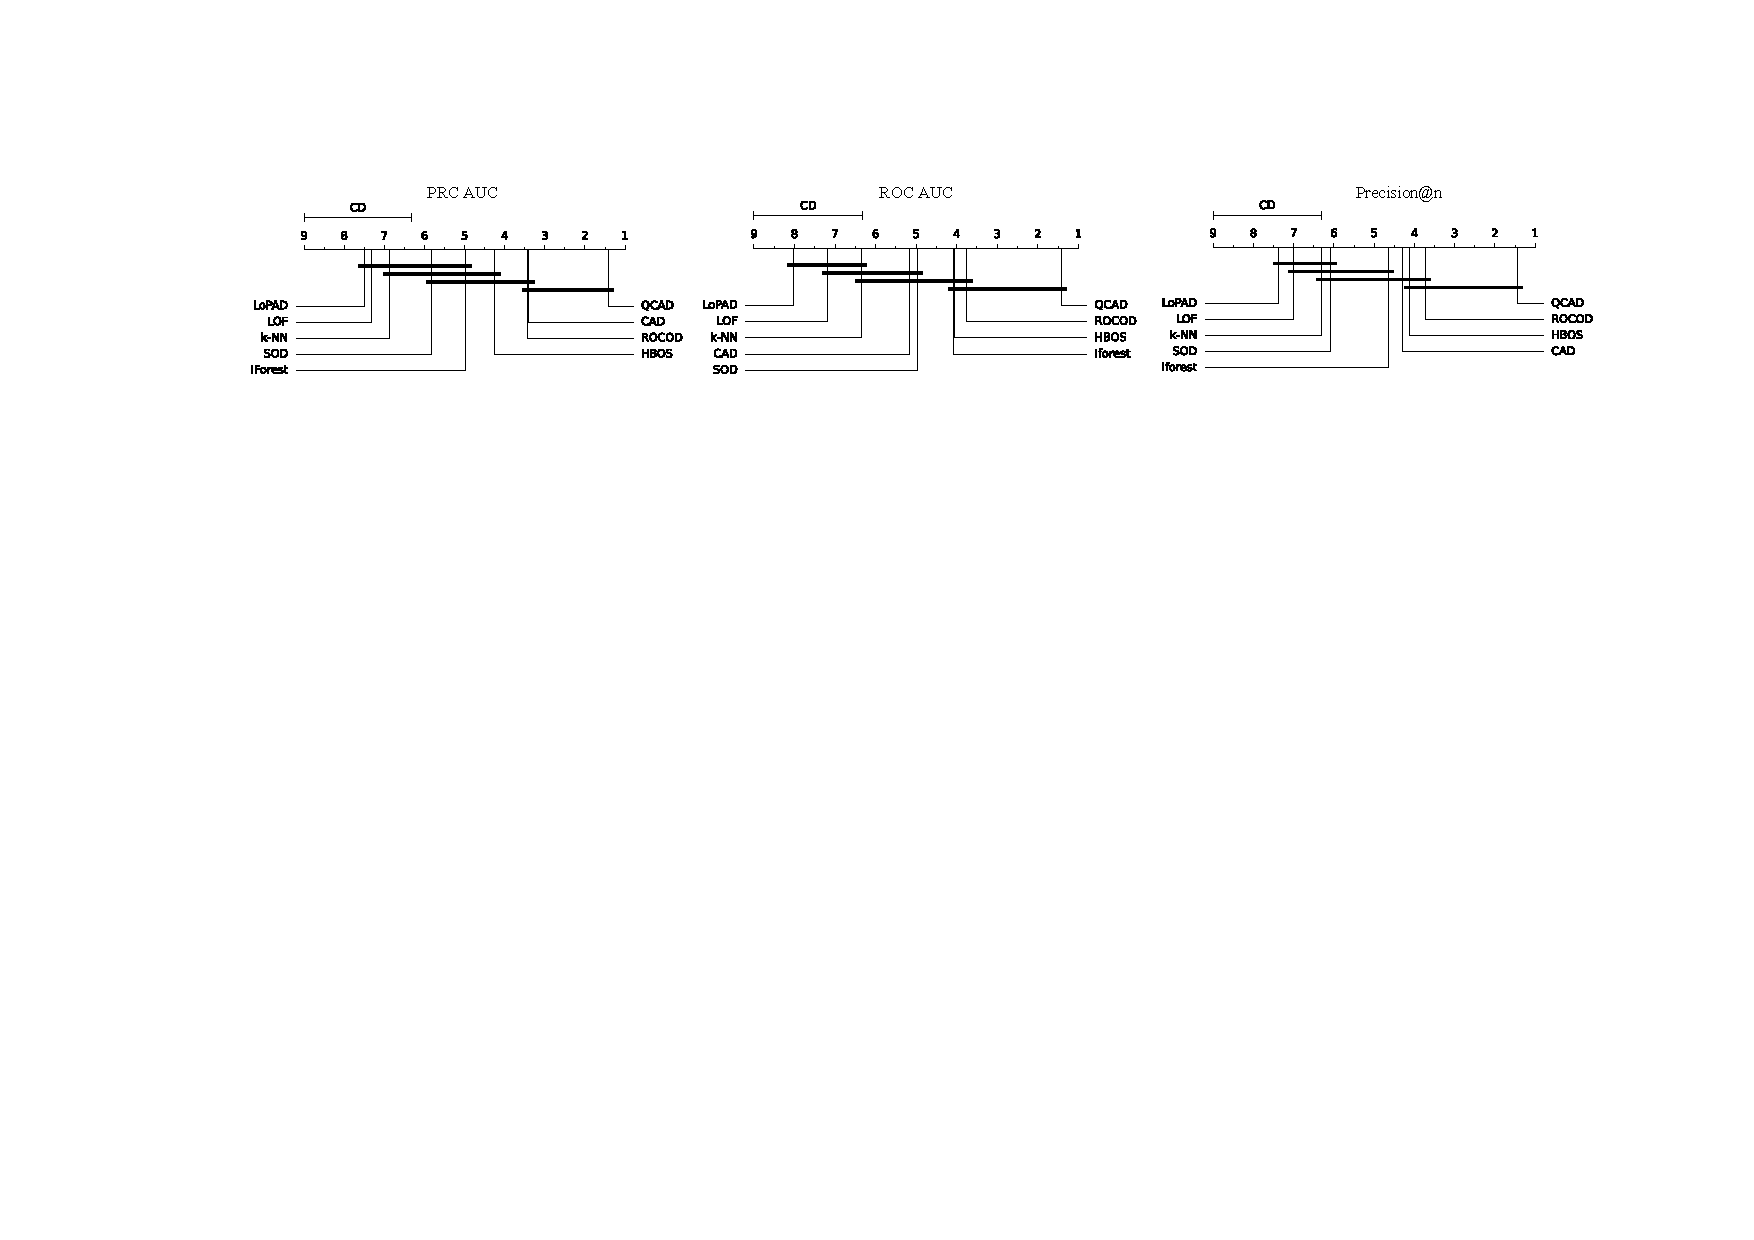
\includegraphics[width=12cm]{images/Pic_StatCom.pdf}
\caption{Biểu đồ khác biệt quan trọng thể hiện sự so sánh khác biệt thống kê giữa QCAD và các đối thủ của nó về PRC AUC, ROC AUC và Precision@n. Để đạt được điều này, chúng tôi sử dụng các bài kiểm tra Friedman \citep{friedman1937use}, sau đó là phân tích hậu kỳ Nemenyi \citep{nemenyi1963distribution} với mức ý nghĩa $0.05$. Thử nghiệm Nemenyi hậu kiểm cho thấy không có sự khác biệt đáng kể trong QCAD, CAD và ROCOD về mặt AUC của PRC; không có sự khác biệt đáng kể trong QCAD, ROCOD, HBOS và IForest về ROC AUC; không có sự khác biệt đáng kể nào trong QCAD, ROCOD, HBOS và CAD về Precision@n. Tuy nhiên, người ta có thể thấy rằng QCAD luôn vượt trội so với các đối thủ của nó ở ba chỉ số.
}\label{fig:StatCom}
\end{figure}We also observe that QCAD performs well on datasets with varying sample size, dimensionality, and rate of injected anomalies. Specifically, QCAD achieved a high ROC AUC ($\ge 0.85$) on all datasets. Giá trị này tốt hơn nhiều so với các giá trị ROC AUC gần với $0.50$ mà ROCOD, CAD, HBOS và IForest thu được trên một số tập dữ liệu, ngụ ý rằng chúng chỉ là phỏng đoán ngẫu nhiên. In addition, QCAD attained high PRC AUC ($\ge 0.8$) and Precision@n values ($\ge 0.7$) on most datasets. The lowest PRC AUC and Precision@n value are is 0.46 and 0.49, respectively, both obtained on the Toxicity dataset. Các lý do có thể dẫn đến hiệu suất vừa phải của QCAD trên Airfoil, BodyFat, Power plant và Toxicity là: mối quan hệ phụ thuộc giữa các đặc trưng hành vi và các đặc điểm ngữ cảnh không chặt chẽ hoặc mối quan hệ phụ thuộc quá phức tạp để Rừng hồi quy phân vị có thể nắm bắt được. Tuy nhiên, ROCOD, COD, HBOS và IForest nhận được các giá trị AUC PRC nhỏ hơn các giá trị 0.70 và Precision@n nhỏ hơn 0.60 trên hầu hết các tập dữ liệu. Moreover, HBOS and IForest sometimes attain PRC AUC and Precision@n lower than 0.10, which is extremely poor. Điều này ngụ ý rằng các phương pháp phát hiện sự bất thường truyền thống không phù hợp để xác định sự bất thường theo ngữ cảnh vì chúng xử lý tất cả các đặc điểm như nhau. Hơn nữa, hiệu suất tương đối kém của ROCOD và CAD---so với phương pháp của chúng tôi---cho thấy tầm quan trọng của việc lập mô hình nhiều thuộc tính của phân bố có điều kiện hơn là chỉ giá trị trung bình.

\subsection{Phân tích thời gian chạy} \label{subsec:runtime}
\begin{figure}[!htbp]
\centering
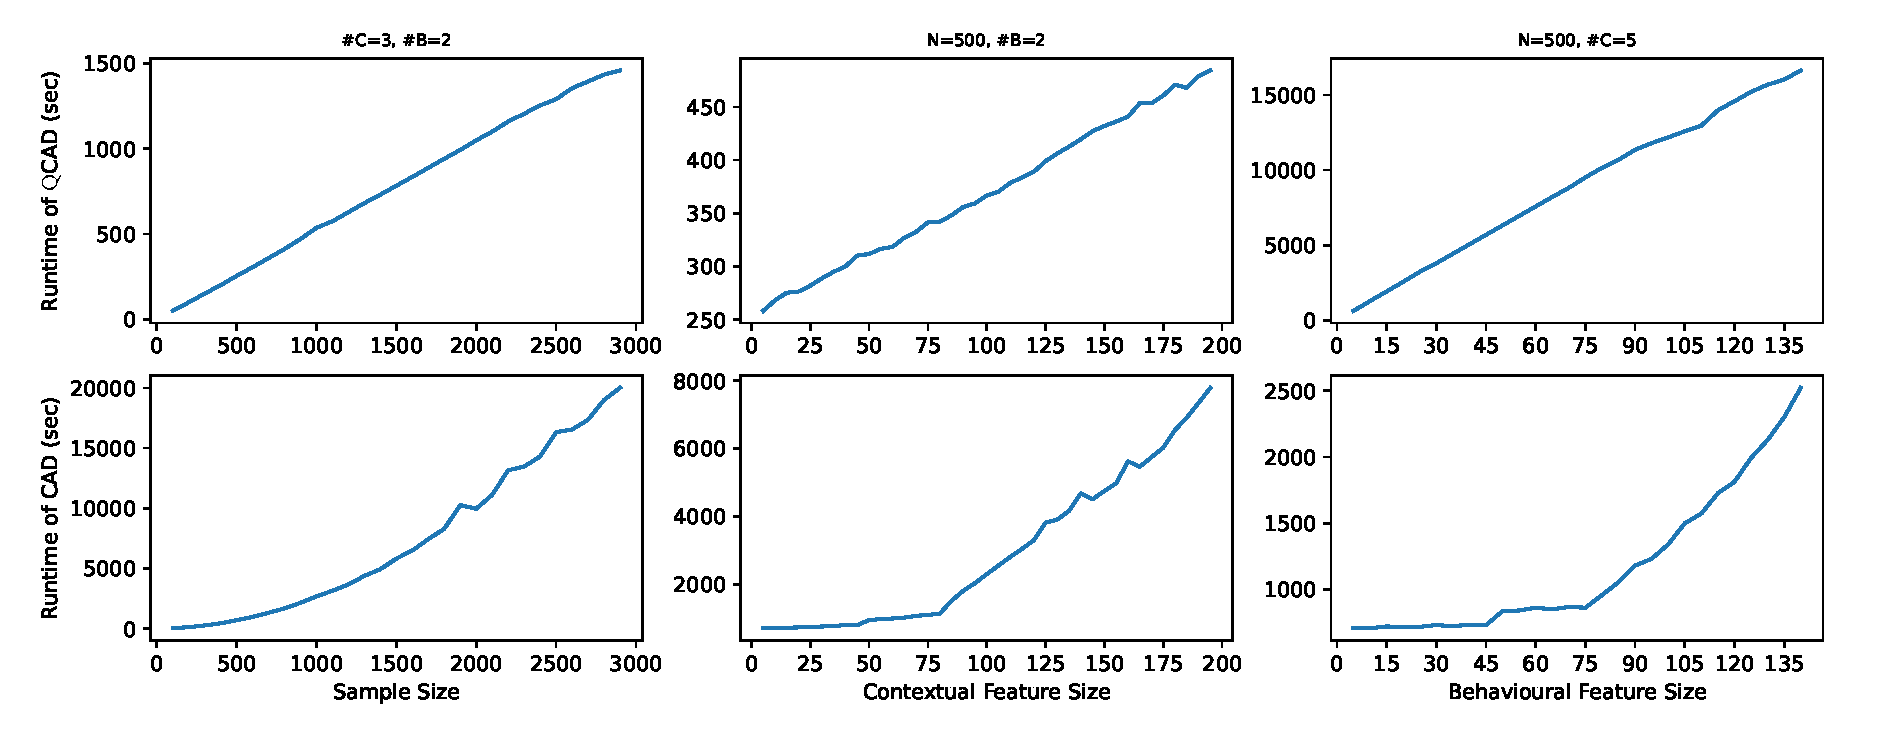
\includegraphics[width=12cm]{images/Pic_runtime.pdf}
\caption{Phân tích thời gian chạy bằng cách thay đổi kích thước mẫu, số lượng đặc trưng ngữ cảnh ($\#\textbf{C}$) và số lượng đặc trưng hành vi ($\#\textbf{B}$). Kết quả thu được từ các thử nghiệm độc lập 5. Dữ liệu được tổng hợp bằng sơ đồ S1. Lưu ý các tỷ lệ trục y khác nhau.}\label{fig:runtime}
\end{figure}

Để điều tra khả năng mở rộng và hiệu quả của QCAD, chúng tôi thực hiện phân tích thời gian chạy bằng cách thay đổi kích thước mẫu, số lượng đặc trưng ngữ cảnh và số lượng đặc trưng hành vi. Như được hiển thị trong Hình ~ \ref{fig:runtime}, chúng ta có thể quan sát bằng thực nghiệm rằng thời gian chạy của QCAD tỷ lệ tuyến tính đối với kích thước mẫu, số lượng đặc trưng ngữ cảnh và số lượng đặc trưng hành vi trên các tập dữ liệu vừa và nhỏ. In contrast, CAD is computationally prohibitively expensive even on small datasets. To further understand the complexity of QCAD, we perform a time complexity analysis in Appendix~\ref{Appendix:Complexity}. The theoretical analysis is in line with our empirical results and analysis.

\subsection{Using QCAD to Find Promising Football Players}
\label{subsec:application}

Trong phần này, chúng tôi minh họa khả năng của QCAD trong việc xác định các bất thường theo ngữ cảnh có ý nghĩa tiềm ẩn và đưa ra các giải thích trực quan và dễ hiểu cho các bất thường được báo cáo khi áp dụng cho một vấn đề trong thế giới thực.\begin{figure}[!htbp]
\centering
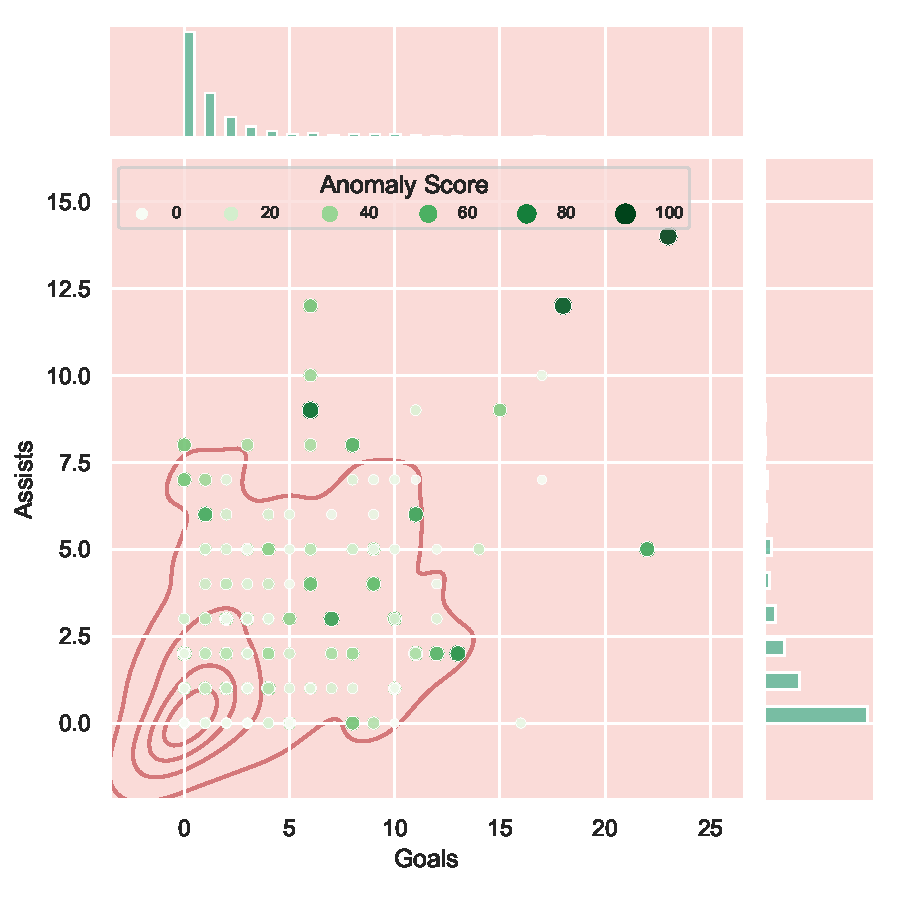
\includegraphics[width=8cm]{images/Pic_football1.pdf}
\caption{Sự phân bố của tất cả người chơi trong không gian hành vi $Assists \times Goals$ và điểm bất thường tương ứng của họ do QCAD đưa ra. Các đường cong màu đỏ biểu thị mật độ ước tính của phân bố chung ở các cấp độ khác nhau, biểu đồ biểu thị phân bố cận biên. Dấu chấm màu xanh lục lớn hơn và đậm hơn biểu thị điểm bất thường lớn hơn do QCAD đưa ra. }\label{fig:football1}
\end{figure}

Trong trường hợp sử dụng, chúng tôi xem xét vấn đề tìm kiếm những cầu thủ xuất sắc ở Giải Ngoại hạng Anh. Tập dữ liệu\footnote{https://www.kaggle.com/rajatrc1705/english-premier-league202021} mô tả thông tin cơ bản và thống kê hiệu suất của các cầu thủ bóng đá 532 từ 2020 đến 2021. Chúng tôi sử dụng các biến \textit{Position1,Position2} (vị trí mà người chơi chơi), \textit{Age} (tuổi của người chơi), \textit{Matches} (số trận đấu đã chơi), \textit{Starts} (số trận đấu mà người chơi có trong đội hình xuất phát) và \textit{Mins} (tổng số phút người chơi đã chơi) dưới dạng các đặc trưng ngữ cảnh. Hai số liệu thống kê về hiệu suất, \textit{Mục tiêu} (số bàn thắng mà cầu thủ ghi được) và \textit{Hỗ trợ} (số đường kiến ​​tạo do cầu thủ thực hiện), được coi là các đặc trưng hành vi.

Hình \ref{fig:football1} mô tả sự phân bố của tất cả các đối tượng dữ liệu trong không gian hành vi $Goals\times Assists$. Không xem xét thông tin theo ngữ cảnh, các máy phát hiện bất thường truyền thống như HBOS, LOF, IForest sẽ coi các vật thể trong khu vực dày đặc (tức là các vật thể nằm bên trong các đường cong màu đỏ) như các vật thể bình thường. Ngược lại, bộ phát hiện bất thường theo ngữ cảnh QCAD của chúng tôi có thể phát hiện các điểm bất thường ở các khu vực dày đặc bằng cách xem xét thông tin theo ngữ cảnh (tức là các vật thể màu xanh lá cây nằm bên trong các đường cong màu đỏ). Cụ thể, Hình~\ref{fig:football1} cũng trình bày điểm bất thường do QCAD đưa ra (với cài đặt mặc định). Ví dụ: người chơi Matheus Pereira---người đã đạt được các mục tiêu 11 và hỗ trợ 6---được QCAD báo cáo là 'bất thường' (tức là có điểm bất thường tương đối cao) nhưng lại là 'bình thường' bởi các máy phát hiện bất thường truyền thống. Ngược lại, QCAD coi Patrick Bamford, một cầu thủ có các bàn thắng 17 và kiến ​​tạo 7 (trong một khu vực thưa thớt), là bình thường, trong khi các máy phát hiện bất thường truyền thống coi anh ta là một kẻ dị thường.


\begin{figure}[!htbp]
\centering
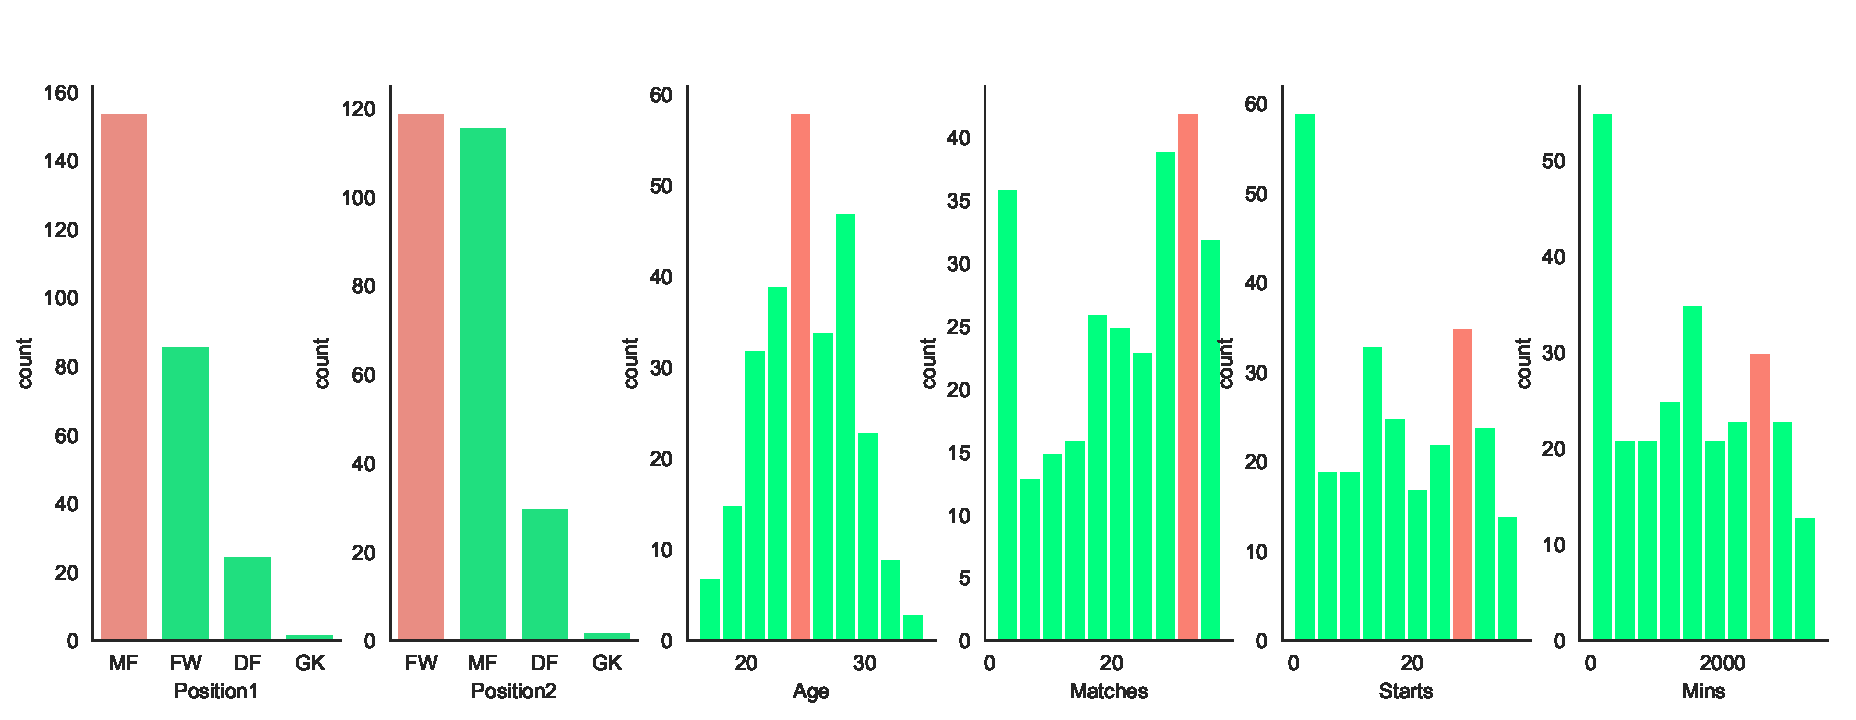
\includegraphics[width=12cm]{images/Pic_football2.pdf}
\caption{Giải thích cho người chơi dị thường được xác định là Matheus Pereira dựa trên nhóm tham chiếu của anh ta. Hiển thị là các giá trị của Matheus Pereira (thùng màu đỏ) liên quan đến việc phân bổ các lân cận theo ngữ cảnh của anh ấy cho từng đặc trưng ngữ cảnh.}\label{fig:football2}
\end{figure}


\begin{figure}[!htbp]
\centering
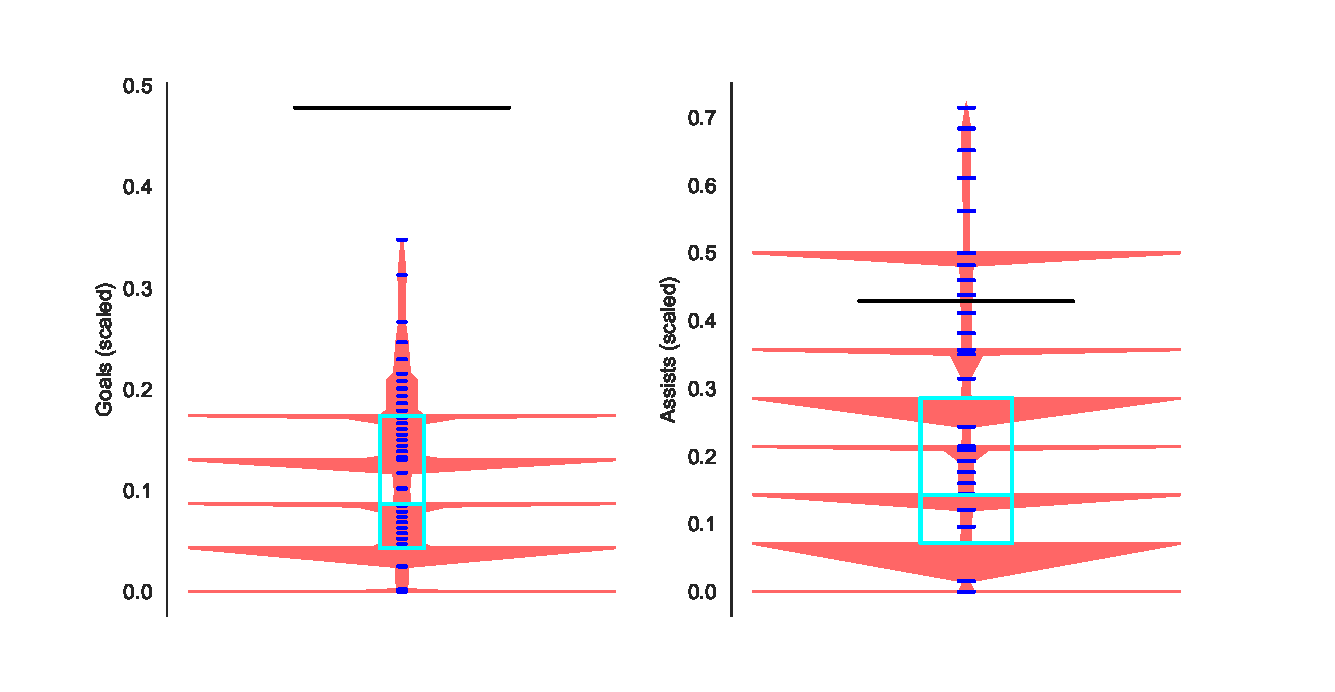
\includegraphics[width=12cm]{images/Pic_football3.pdf}
\caption{Giải thích lý do tại sao Matheus Pereira được coi là một điều bất thường: đặc biệt có nhiều bàn thắng so với những cầu thủ có bối cảnh tương tự và tương đối nhiều đường kiến tạo. Beanplot hiển thị mức phân bổ có điều kiện ước tính của từng đặc trưng hành vi, với vùng màu đỏ rộng hơn biểu thị xác suất xảy ra cao hơn. Các đường ngang màu đen biểu thị các giá trị được báo cáo cho người chơi đang được điều tra.}\label{fig:football3}
\end{figure}Ngoài việc đưa ra điểm bất thường cho từng đối tượng dữ liệu, QCAD cũng có thể đưa ra lời giải thích. Ví dụ: đối với Matheus Pereira ($Position1$ = "MF", $Position2$ = "FW", $Age$=24, $Matches$=33, $Starts$=30, $Mins$=2577), Hình~\ref{fig:football2} hiển thị sự phân bổ giá trị của từng đặc điểm ngữ cảnh cho tất cả người chơi trong vùng lân cận theo ngữ cảnh của anh ta (tức là những người chơi tương tự). Có thể thấy, hầu hết những cầu thủ này đều là Tiền vệ (MF) và/hoặc Tiền đạo (FW), có độ tuổi từ 22 đến 28, thi đấu nhiều trận hơn 25 lần, v.v. Điểm dị thường là 65.8, đưa cầu thủ này vào top-$10$ của hầu hết các cầu thủ dị thường. Điểm này có thể được phân tách theo các đặc trưng hành vi để đưa ra (các) đặc trưng hành vi đóng góp nhiều nhất vào điểm bất thường thu được; \emph{Mục tiêu}, trong trường hợp này. Hơn nữa, Hình~\ref{fig:football3} cho thấy cách trực quan hóa giống như Beanplot có thể giúp cung cấp cái nhìn sâu sắc về cách các giá trị đặc trưng hành vi khác với các giá trị trong vùng lân cận theo ngữ cảnh của người chơi. Từ những biểu đồ này, chúng ta có thể thấy rằng Matheus Pereira đặc biệt giỏi trong việc ghi bàn và tốt hơn một chút so với mong đợi về khả năng kiến ​​tạo.

Những kết quả này có thể được hiểu là: Matheus Pereira thể hiện tốt một cách đáng ngạc nhiên về số bàn thắng và tốt hơn một chút so với mong đợi về số lần kiến ​​tạo khi so sánh với các tiền vệ và/hoặc tiền đạo khác ở độ tuổi 22-28, người đã chơi nhiều hơn 25 số phút và chơi nhiều hơn 2000 số phút. Mặc dù chúng tôi không phải là chuyên gia bóng đá, nhưng chúng tôi hy vọng tính năng phát hiện tự động và giải thích tỷ số có thể hiểu được về những 'bất thường' như vậy sẽ có ý nghĩa và có thể hữu ích cho các huấn luyện viên và tuyển trạch viên bóng đá.
